% Options for packages loaded elsewhere
\PassOptionsToPackage{unicode}{hyperref}
\PassOptionsToPackage{hyphens}{url}
%
\documentclass[
]{article}
\usepackage{amsmath,amssymb}
\usepackage{lmodern}
\usepackage{iftex}
\ifPDFTeX
  \usepackage[T1]{fontenc}
  \usepackage[utf8]{inputenc}
  \usepackage{textcomp} % provide euro and other symbols
\else % if luatex or xetex
  \usepackage{unicode-math}
  \defaultfontfeatures{Scale=MatchLowercase}
  \defaultfontfeatures[\rmfamily]{Ligatures=TeX,Scale=1}
\fi
% Use upquote if available, for straight quotes in verbatim environments
\IfFileExists{upquote.sty}{\usepackage{upquote}}{}
\IfFileExists{microtype.sty}{% use microtype if available
  \usepackage[]{microtype}
  \UseMicrotypeSet[protrusion]{basicmath} % disable protrusion for tt fonts
}{}
\makeatletter
\@ifundefined{KOMAClassName}{% if non-KOMA class
  \IfFileExists{parskip.sty}{%
    \usepackage{parskip}
  }{% else
    \setlength{\parindent}{0pt}
    \setlength{\parskip}{6pt plus 2pt minus 1pt}}
}{% if KOMA class
  \KOMAoptions{parskip=half}}
\makeatother
\usepackage{xcolor}
\usepackage[margin=1in]{geometry}
\usepackage{color}
\usepackage{fancyvrb}
\newcommand{\VerbBar}{|}
\newcommand{\VERB}{\Verb[commandchars=\\\{\}]}
\DefineVerbatimEnvironment{Highlighting}{Verbatim}{commandchars=\\\{\}}
% Add ',fontsize=\small' for more characters per line
\usepackage{framed}
\definecolor{shadecolor}{RGB}{248,248,248}
\newenvironment{Shaded}{\begin{snugshade}}{\end{snugshade}}
\newcommand{\AlertTok}[1]{\textcolor[rgb]{0.94,0.16,0.16}{#1}}
\newcommand{\AnnotationTok}[1]{\textcolor[rgb]{0.56,0.35,0.01}{\textbf{\textit{#1}}}}
\newcommand{\AttributeTok}[1]{\textcolor[rgb]{0.77,0.63,0.00}{#1}}
\newcommand{\BaseNTok}[1]{\textcolor[rgb]{0.00,0.00,0.81}{#1}}
\newcommand{\BuiltInTok}[1]{#1}
\newcommand{\CharTok}[1]{\textcolor[rgb]{0.31,0.60,0.02}{#1}}
\newcommand{\CommentTok}[1]{\textcolor[rgb]{0.56,0.35,0.01}{\textit{#1}}}
\newcommand{\CommentVarTok}[1]{\textcolor[rgb]{0.56,0.35,0.01}{\textbf{\textit{#1}}}}
\newcommand{\ConstantTok}[1]{\textcolor[rgb]{0.00,0.00,0.00}{#1}}
\newcommand{\ControlFlowTok}[1]{\textcolor[rgb]{0.13,0.29,0.53}{\textbf{#1}}}
\newcommand{\DataTypeTok}[1]{\textcolor[rgb]{0.13,0.29,0.53}{#1}}
\newcommand{\DecValTok}[1]{\textcolor[rgb]{0.00,0.00,0.81}{#1}}
\newcommand{\DocumentationTok}[1]{\textcolor[rgb]{0.56,0.35,0.01}{\textbf{\textit{#1}}}}
\newcommand{\ErrorTok}[1]{\textcolor[rgb]{0.64,0.00,0.00}{\textbf{#1}}}
\newcommand{\ExtensionTok}[1]{#1}
\newcommand{\FloatTok}[1]{\textcolor[rgb]{0.00,0.00,0.81}{#1}}
\newcommand{\FunctionTok}[1]{\textcolor[rgb]{0.00,0.00,0.00}{#1}}
\newcommand{\ImportTok}[1]{#1}
\newcommand{\InformationTok}[1]{\textcolor[rgb]{0.56,0.35,0.01}{\textbf{\textit{#1}}}}
\newcommand{\KeywordTok}[1]{\textcolor[rgb]{0.13,0.29,0.53}{\textbf{#1}}}
\newcommand{\NormalTok}[1]{#1}
\newcommand{\OperatorTok}[1]{\textcolor[rgb]{0.81,0.36,0.00}{\textbf{#1}}}
\newcommand{\OtherTok}[1]{\textcolor[rgb]{0.56,0.35,0.01}{#1}}
\newcommand{\PreprocessorTok}[1]{\textcolor[rgb]{0.56,0.35,0.01}{\textit{#1}}}
\newcommand{\RegionMarkerTok}[1]{#1}
\newcommand{\SpecialCharTok}[1]{\textcolor[rgb]{0.00,0.00,0.00}{#1}}
\newcommand{\SpecialStringTok}[1]{\textcolor[rgb]{0.31,0.60,0.02}{#1}}
\newcommand{\StringTok}[1]{\textcolor[rgb]{0.31,0.60,0.02}{#1}}
\newcommand{\VariableTok}[1]{\textcolor[rgb]{0.00,0.00,0.00}{#1}}
\newcommand{\VerbatimStringTok}[1]{\textcolor[rgb]{0.31,0.60,0.02}{#1}}
\newcommand{\WarningTok}[1]{\textcolor[rgb]{0.56,0.35,0.01}{\textbf{\textit{#1}}}}
\usepackage{graphicx}
\makeatletter
\def\maxwidth{\ifdim\Gin@nat@width>\linewidth\linewidth\else\Gin@nat@width\fi}
\def\maxheight{\ifdim\Gin@nat@height>\textheight\textheight\else\Gin@nat@height\fi}
\makeatother
% Scale images if necessary, so that they will not overflow the page
% margins by default, and it is still possible to overwrite the defaults
% using explicit options in \includegraphics[width, height, ...]{}
\setkeys{Gin}{width=\maxwidth,height=\maxheight,keepaspectratio}
% Set default figure placement to htbp
\makeatletter
\def\fps@figure{htbp}
\makeatother
\setlength{\emergencystretch}{3em} % prevent overfull lines
\providecommand{\tightlist}{%
  \setlength{\itemsep}{0pt}\setlength{\parskip}{0pt}}
\setcounter{secnumdepth}{-\maxdimen} % remove section numbering
\ifLuaTeX
  \usepackage{selnolig}  % disable illegal ligatures
\fi
\IfFileExists{bookmark.sty}{\usepackage{bookmark}}{\usepackage{hyperref}}
\IfFileExists{xurl.sty}{\usepackage{xurl}}{} % add URL line breaks if available
\urlstyle{same} % disable monospaced font for URLs
\hypersetup{
  hidelinks,
  pdfcreator={LaTeX via pandoc}}

\author{}
\date{\vspace{-2.5em}}

\begin{document}

\textbf{University of Edinburgh}

\textbf{School of Mathematics}

\textbf{Bayesian Data Analysis, 2022/2023, Semester 2}

\textbf{Assignment 1}

\textbf{IMPORTANT INFORMATION ABOUT THE ASSIGNMENT}

\textbf{In this paragraph, we summarize the essential information about
this assignment. The format and rules for this assignment are different
from your other courses, so please pay attention.}

\textbf{1) Deadline: The deadline for submitting your solutions to this
assignment is the 6 March 12:00 noon Edinburgh time.}

\textbf{2) Format: You will need to submit your work as 2 components: a
PDF report, and your R Markdown (.Rmd) notebook. There will be two
separate submission systems on Learn: Gradescope for the report in PDF
format, and a Learn assignment for the code in Rmd format. You need to
write your solutions into this R Markdown notebook (code in R chunks and
explanations in Markdown chunks), and then select Knit/Knit to PDF in
RStudio to create a PDF report.}

\includegraphics[width=2in,height=\textheight]{knit_to_PDF.jpg}

\textbf{The compiled PDF needs to contain everything in this notebook,
with your code sections clearly visible (not hidden), and the output of
your code included. Reports without the code displayed in the PDF, or
without the output of your code included in the PDF will be marked as 0,
with the only feedback ``Report did not meet submission requirements''.}

\textbf{You need to upload this PDF in Gradescope submission system, and
your Rmd file in the Learn assignment submission system. You will be
required to tag every sub question on Gradescope.}

\textbf{Some key points that are different from other courses:}

\textbf{a) Your report needs to contain written explanation for each
question that you solve, and some numbers or plots showing your results.
Solutions without written explanation that clearly demonstrates that you
understand what you are doing will be marked as 0 irrespectively whether
the numerics are correct or not.}

\textbf{b) Your code has to be possible to run for all questions by the
Run All in RStudio, and reproduce all of the numerics and plots in your
report (up to some small randomness due to stochasticity of Monte Carlo
simulations). The parts of the report that contain material that is not
reproduced by the code will not be marked (i.e.~the score will be 0),
and the only feedback in this case will be that the results are not
reproducible from the code.}

\includegraphics[width=3.90625in,height=\textheight]{run_all.jpg}

\textbf{c) Multiple Submissions are allowed BEFORE THE DEADLINE are
allowed for both the report, and the code.\\
However, multiple submissions are NOT ALLOWED AFTER THE DEADLINE.\\
YOU WILL NOT BE ABLE TO MAKE ANY CHANGES TO YOUR SUBMISSION AFTER THE
DEADLINE.\\
Nevertheless, if you did not submit anything before the deadline, then
you can still submit your work after the deadline, but late penalties
will apply. The timing of the late penalties will be determined by the
time you have submitted BOTH the report, and the code (i.e.~whichever
was submitted later counts).}

\textbf{We illustrate these rules by some examples:}

\textbf{Alice has spent a lot of time and effort on her assignment for
BDA. Unfortunately she has accidentally introduced a typo in her code in
the first question, and it did not run using Run All in RStudio. - Alice
will get 0 for the whole assignment, with the only feedback ``Results
are not reproducible from the code''.}

\textbf{Bob has spent a lot of time and effort on his assignment for
BDA. Unfortunately he forgot to submit his code. - Bob will get no
personal reminder to submit his code. Bob will get 0 for the whole
assignment, with the only feedback ``Results are not reproducible from
the code, as the code was not submitted.''}

\textbf{Charles has spent a lot of time and effort on his assignment for
BDA. He has submitted both his code and report in the correct formats.
However, he did not include any explanations in the report. Charles will
get 0 for the whole assignment, with the only feedback ``Explanation is
missing.''}

\textbf{Denise has spent a lot of time and effort on her assignment for
BDA. She has submitted her report in the correct format, but thought
that she can include her code as a link in the report, and upload it
online (such as Github, or Dropbox). - Denise will get 0 for the whole
assignment, with the only feedback ``Code was not uploaded on Learn.''}

\textbf{3) Group work: This is an INDIVIDUAL ASSIGNMENT, like a 2 week
exam for the course. Communication between students about the assignment
questions is not permitted. Students who submit work that has not been
done individually will be reported for Academic Misconduct, that can
lead to serious consequences. Each problem will be marked by a single
instructor, so we will be able to spot students who copy.}

\textbf{4) Piazza: During the periods of the assignments, the instructor
will change Piazza to allow messaging the instructors only,
i.e.~students will not see each others messages and replies.}

\textbf{Only questions regarding clarification of the statement of the
problems will be answered by the instructors. The instructors will not
give you any information related to the solution of the problems, such
questions will be simply answered as ``This is not about the statement
of the problem so we cannot answer your question.''}

\textbf{THE INSTRUCTORS ARE NOT GOING TO DEBUG YOUR CODE, AND YOU ARE
ASSESSED ON YOUR ABILITY TO RESOLVE ANY CODING OR TECHNICAL DIFFICULTIES
THAT YOU ENCOUNTER ON YOUR OWN.}

\textbf{5) Office hours: There will be two office hours per week (Monday
14:00-15:00, and Wednesdays 15:00-16:00) during the 2 weeks for this
assignment. The links are available on Learn / Course Information. I
will be happy to discuss the course/workshop materials. However, I will
only answer questions about the assignment that require clarifying the
statement of the problems, and will not give you any information about
the solutions. Students who ask for feedback on their assignment
solutions during office hours will be removed from the meeting.}

\textbf{6) Late submissions and extensions: NO EXTENSIONS ARE ALLOWED
FOR THIS ASSIGNMENT, AND THERE IS NO SUCH OPTION PROVIDED IN THE ESC
SYSTEM. Students who have existing Learning Adjustments in Euclid will
be allowed to have the same adjustments applied to this course as well,
but they need to apply for this BEFORE THE DEADLINE on the website}

\url{https://www.ed.ac.uk/student-administration/extensions-special-circumstances}

\textbf{by clicking on ``Access your learning adjustment''. This will be
approved automatically.}

\textbf{Students who submit their work late will have late submission
penalties applied by the ESC team automatically (this means that even if
you are 1 second late because of your internet connection was slow, the
penalties will still apply). The penalties are 5\% of the total mark
deduced for every day of delay started (i.e.~one minute of delay counts
for 1 day). The course instructors do not have any role in setting these
penalties, we will not be able to change them.}

\begin{Shaded}
\begin{Highlighting}[]
\FunctionTok{rm}\NormalTok{(}\AttributeTok{list =} \FunctionTok{ls}\NormalTok{(}\AttributeTok{all =} \ConstantTok{TRUE}\NormalTok{))}
\CommentTok{\#Do not delete this!}
\CommentTok{\#It clears all variables to ensure reproducibility}
\end{Highlighting}
\end{Shaded}

\includegraphics{Exchange-rate.jpg}

\textbf{Problem 1}

\textbf{In this problem, we study a dataset about currency exchange
rates. The exrates dataset of the stochvol package contains the daily
average exchange rates of 24 currencies versus the EUR, from 2000-01-03
until 2012-04-04.}

\begin{Shaded}
\begin{Highlighting}[]
\FunctionTok{require}\NormalTok{(stochvol)}
\end{Highlighting}
\end{Shaded}

\begin{verbatim}
## Loading required package: stochvol
\end{verbatim}

\begin{Shaded}
\begin{Highlighting}[]
\FunctionTok{data}\NormalTok{(}\StringTok{"exrates"}\NormalTok{)}
\CommentTok{\#You may need to set the working directory first before loading the dataset}
\CommentTok{\#setwd("location of Assignment 1")}
\CommentTok{\#The first 6 rows of the dataframe}
\FunctionTok{print.data.frame}\NormalTok{(exrates[}\DecValTok{1}\SpecialCharTok{:}\DecValTok{6}\NormalTok{,])}
\end{Highlighting}
\end{Shaded}

\begin{verbatim}
##               AUD    CAD    CHF    CZK    DKK    GBP    HKD     IDR    JPY
## 2000/01/03 1.5346 1.4577 1.6043 36.063 7.4404 0.6246 7.8624 7133.32 102.75
## 2000/01/04 1.5677 1.4936 1.6053 36.270 7.4429 0.6296 8.0201 7265.16 105.88
## 2000/01/05 1.5773 1.5065 1.6060 36.337 7.4444 0.6324 8.0629 7437.97 107.34
## 2000/01/06 1.5828 1.5091 1.6068 36.243 7.4441 0.6302 8.0843 7495.52 108.72
## 2000/01/07 1.5738 1.5010 1.6079 36.027 7.4436 0.6262 8.0030 7398.88 108.09
## 2000/01/10 1.5587 1.4873 1.6089 35.988 7.4448 0.6249 7.9471 7320.49 107.26
##                KRW    MXN    MYR    NOK    NZD    PHP    PLN    RON     RUB
## 2000/01/03 1140.02 9.6105 3.8422 8.0620 1.9331 40.424 4.1835 1.8273 27.7548
## 2000/01/04 1157.32 9.7453 3.9188 8.1500 1.9745 40.992 4.2423 1.8858 28.3594
## 2000/01/05 1176.08 9.8969 3.9393 8.2060 1.9956 41.637 4.2627 1.8979 28.3006
## 2000/01/06 1191.90 9.9751 3.9498 8.2030 2.0064 42.148 4.2593 1.9000 28.5111
## 2000/01/07 1169.52 9.8368 3.9100 8.1945 1.9942 41.493 4.1897 1.8822 28.2526
## 2000/01/10 1157.84 9.6449 3.8824 8.1900 1.9783 41.226 4.1567 1.8729 28.7609
##               SEK    SGD     THB      TRY    USD       date
## 2000/01/03 8.5520 1.6769 37.2793 0.546131 1.0090 2000-01-03
## 2000/01/04 8.6215 1.7047 38.2078 0.552354 1.0305 2000-01-04
## 2000/01/05 8.6415 1.7159 38.5375 0.555329 1.0368 2000-01-05
## 2000/01/06 8.6445 1.7291 39.0734 0.555674 1.0388 2000-01-06
## 2000/01/07 8.6450 1.7096 38.4299 0.554980 1.0284 2000-01-07
## 2000/01/10 8.6570 1.6975 38.0328 0.552469 1.0229 2000-01-10
\end{verbatim}

\begin{Shaded}
\begin{Highlighting}[]
\FunctionTok{cat}\NormalTok{(}\FunctionTok{paste}\NormalTok{(}\StringTok{"Data from "}\NormalTok{, }\FunctionTok{min}\NormalTok{(exrates}\SpecialCharTok{$}\NormalTok{date),}\StringTok{" until "}\NormalTok{,}\FunctionTok{max}\NormalTok{(exrates}\SpecialCharTok{$}\NormalTok{date)))}
\end{Highlighting}
\end{Shaded}

\begin{verbatim}
## Data from  2000-01-03  until  2012-04-04
\end{verbatim}

\textbf{As we can see, not all dates are included in the dataset. Some
are missing, such as weekends, and public holidays.}

\textbf{In this problem, we are going to fit a various stochastic
volatility models on this dataset (see e.g.
\url{https://www.jstor.org/stable/1392251}).}

\textbf{a){[}10 marks{]} Consider the following leveraged Stochastic
Volatility (SV) model.}

\(\begin{aligned} y_t&=\beta_0+\beta_1 y_{t-1}+\exp(h_t/2)\epsilon_t \quad \text{for}\quad 1\le t\le T,\\ h_{t+1}&=\mu+\phi(h_t-\mu)+\sigma \eta_t\quad \text{for} \quad 0\le t\le T, \quad h_0\sim N(\mu, \sigma^2/(1-\phi^2)),\\(\epsilon_t,\eta_t)&\sim N\left(0, \Sigma_{\rho}\right)\quad \text{ for } \quad \Sigma_{\rho}=\left(\begin{matrix}1 & \rho\\ \rho & 1\end{matrix}\right). \end{aligned}\)

\textbf{Here} \(t\) \textbf{is the time index,} \(y_t\) \textbf{are the
observations (such as daily USD/EUR rate),} \(h_t\) \textbf{are the
log-variance process,} \(\epsilon_t\) \textbf{is the observation noise,
and} \(\eta_t\) \textbf{is the log-variance process noise (which are
correlated, but independent for different values of} \$t\$\textbf{). The
hyperparameters are}
\(\beta_0, \beta_1, \mu, \phi, \sigma, \rho\)\textbf{.}

\textbf{For stability, it is necessary to have}
\(\phi\in (-1,1)\)\textbf{, and by the definition of correlation
matrices, we have} \(\rho\in [-1,1]\)\textbf{.}

\textbf{Implement this model in JAGS or Stan on the first 3 months of
USD/EUR data from the dataset, i.e.~from dates 2000-01-03 until
2000-04-02.}

\textbf{Explain how did you choose priors for all parameters. Explain
how did you take into account the days without observation in your
model.}

\textbf{Fit the model, do convergence diagnostics, print out the summary
of the results, and discuss them.}

\textbf{Make sure that the Effective Sample Size is at least 1000 for
all 6 hyperparameters (you need to choose burn-in and number of steps
appropriately for this).}

\begin{Shaded}
\begin{Highlighting}[]
\DocumentationTok{\#\# Loading JAGS}
\FunctionTok{require}\NormalTok{(rjags)}
\end{Highlighting}
\end{Shaded}

\begin{verbatim}
## Loading required package: rjags
\end{verbatim}

\begin{verbatim}
## Loading required package: coda
\end{verbatim}

\begin{verbatim}
## Linked to JAGS 4.3.1
\end{verbatim}

\begin{verbatim}
## Loaded modules: basemod,bugs
\end{verbatim}

\begin{Shaded}
\begin{Highlighting}[]
\DocumentationTok{\#\# We want to extract the data from the USD/EUR and the GBP/EUR(used in a later}
\DocumentationTok{\#\# question) pair corresponding to dates from 2000{-}01{-}03 to 2000{-}04{-}02, but is }
\DocumentationTok{\#\# evident that 2000{-}04{-}02 lies on a weekend, so it is one of the dates missing}
\DocumentationTok{\#\# from our data set. We shall define a new vector containing all}
\DocumentationTok{\#\# (including weekends and holidays) and based on that we add NA values}
\DocumentationTok{\#\# for all the exchange rates whose dates were not initially present.}
\DocumentationTok{\#\# As we have seen the lectures JAGS is able to take care of NA values.}

\DocumentationTok{\#\# Extracting usd\_eur forex pair}
\NormalTok{usd\_eur }\OtherTok{\textless{}{-}}\NormalTok{ exrates}\SpecialCharTok{$}\NormalTok{USD}

\DocumentationTok{\#\# Extracting gbp\_eur forex pair}
\NormalTok{gbp\_eur }\OtherTok{\textless{}{-}}\NormalTok{ exrates}\SpecialCharTok{$}\NormalTok{GBP}

\DocumentationTok{\#\# Extracting dates}
\NormalTok{dates }\OtherTok{\textless{}{-}}\NormalTok{ exrates}\SpecialCharTok{$}\NormalTok{date}


\DocumentationTok{\#\# Extracting the positions of the dates that interest us }
\NormalTok{pos1 }\OtherTok{\textless{}{-}} \FunctionTok{which}\NormalTok{(dates}\SpecialCharTok{==}\StringTok{\textquotesingle{}2000{-}01{-}03\textquotesingle{}}\NormalTok{)}
\DocumentationTok{\#\# Final date included before 2000{-}04{-}02 (it\textquotesingle{}s a Friday)}
\NormalTok{pos2 }\OtherTok{\textless{}{-}} \FunctionTok{which}\NormalTok{(dates}\SpecialCharTok{==}\StringTok{\textquotesingle{}2000{-}03{-}31\textquotesingle{}}\NormalTok{)}

\DocumentationTok{\#\# Generating the full sequence of dates}
\NormalTok{full\_dates }\OtherTok{\textless{}{-}} \FunctionTok{seq}\NormalTok{(}\FunctionTok{as.Date}\NormalTok{(}\StringTok{\textquotesingle{}2000{-}01{-}03\textquotesingle{}}\NormalTok{), }\FunctionTok{as.Date}\NormalTok{(}\StringTok{\textquotesingle{}2000{-}04{-}02\textquotesingle{}}\NormalTok{), }\AttributeTok{by=}\StringTok{"days"}\NormalTok{)}

\DocumentationTok{\#\# Keeping only the dates of interest in the initial vector}
\NormalTok{dates }\OtherTok{\textless{}{-}}\NormalTok{ dates[pos1}\SpecialCharTok{:}\NormalTok{pos2]}

\DocumentationTok{\#\# Obtaining the index of observed values}
\NormalTok{ind }\OtherTok{\textless{}{-}} \FunctionTok{c}\NormalTok{()}

\ControlFlowTok{for}\NormalTok{(i }\ControlFlowTok{in} \FunctionTok{seq}\NormalTok{(}\DecValTok{1}\SpecialCharTok{:}\FunctionTok{length}\NormalTok{(dates)))\{}
  
\NormalTok{  ind[i] }\OtherTok{\textless{}{-}} \FunctionTok{which}\NormalTok{(dates[i]}\SpecialCharTok{==}\NormalTok{full\_dates)}
  
\NormalTok{\}}

\DocumentationTok{\#\# Final vector of observations with NA values for weekends and holidays}

\NormalTok{y\_usd }\OtherTok{\textless{}{-}} \FunctionTok{rep}\NormalTok{(}\ConstantTok{NA}\NormalTok{,}\FunctionTok{length}\NormalTok{(full\_dates))}
\NormalTok{y\_gbp }\OtherTok{\textless{}{-}} \FunctionTok{rep}\NormalTok{(}\ConstantTok{NA}\NormalTok{,}\FunctionTok{length}\NormalTok{(full\_dates))}
\NormalTok{usd\_eur }\OtherTok{\textless{}{-}}\NormalTok{ usd\_eur[pos1}\SpecialCharTok{:}\NormalTok{pos2]}
\NormalTok{gbp\_eur }\OtherTok{\textless{}{-}}\NormalTok{ usd\_eur[pos1}\SpecialCharTok{:}\NormalTok{pos2]}
\NormalTok{y\_usd[ind] }\OtherTok{\textless{}{-}}\NormalTok{ usd\_eur}
\NormalTok{y\_gbp[ind] }\OtherTok{\textless{}{-}}\NormalTok{ usd\_eur}


\DocumentationTok{\#\# Total number of days, needed for model compilation}
\NormalTok{n }\OtherTok{\textless{}{-}} \FunctionTok{length}\NormalTok{(y\_usd)}

\DocumentationTok{\#\# Mean of the observations, excluding NA values}
\DocumentationTok{\#\# We will use the mean for centering our observations to help convergence}
\NormalTok{meanY }\OtherTok{\textless{}{-}} \FunctionTok{mean}\NormalTok{(usd\_eur)}
\end{Highlighting}
\end{Shaded}

\begin{Shaded}
\begin{Highlighting}[]
\DocumentationTok{\#\# Below we declare our model in JAGS, the hyperparameters for which we need  }
\DocumentationTok{\#\# to define a prior are :: b0,b1,mu,phi,rho,sigma. We also have to set priors}
\DocumentationTok{\#\# for the initial values of the yt and ht processes}
  
\NormalTok{model\_string\_q1a }\OtherTok{\textless{}{-}} \StringTok{" model\{}
\StringTok{  }
\StringTok{  \#\# Priors for hyperparameters}
\StringTok{  }
\StringTok{  mu \textasciitilde{} dnorm(0,1e{-}4)}
\StringTok{  phi \textasciitilde{} dunif({-}0.99999, 0.99999)}
\StringTok{  rho \textasciitilde{} dunif({-}1, 1)}
\StringTok{  }
\StringTok{  }
\StringTok{  tau \textasciitilde{} dgamma(0.1,0.1)}
\StringTok{  sigma2 \textless{}{-} 1/tau}
\StringTok{  sigma \textless{}{-} sqrt(sigma2)}
\StringTok{  }
\StringTok{  b\_0 \textasciitilde{} dnorm(0, 1e{-}5)}
\StringTok{  b\_1 \textasciitilde{} dnorm(0, 1e{-}5)}
\StringTok{  }
\StringTok{  \#\# Priors for initialiasations}
\StringTok{  }
\StringTok{  eta[1] \textasciitilde{} dnorm(0,1)}
\StringTok{  }
\StringTok{  \#\# We do this so we can write everything in one loop starting from t=2}
\StringTok{  }
\StringTok{  \#\# h[1]}
\StringTok{  h\_0 \textasciitilde{} dnorm(mu, tau1)}
\StringTok{  tau1 \textless{}{-} (1{-}phi*phi)/sigma2}
\StringTok{  mu\_h[1] \textless{}{-} mu + phi*(h\_0{-}mu) + sigma*eta[1]}
\StringTok{  h[1] \textasciitilde{} dnorm(mu\_h[1],tau)}
\StringTok{  }
\StringTok{  \#\# y[1]}
\StringTok{  y\_0 \textasciitilde{} dnorm(0,1e{-}4)}
\StringTok{  mu\_y[1] \textless{}{-} b\_0 + b\_1*(y\_0{-}meanY) + rho*eta[1]*exp(h[1]/2)}
\StringTok{  y[1] \textasciitilde{} dnorm(mu\_y[1],(exp({-}h[1])/(1{-}rho*rho))) }
\StringTok{  y\_rep[1] \textasciitilde{} dnorm(mu\_y[1],(exp({-}h[1])/(1{-}rho*rho)))}
\StringTok{  }
\StringTok{  \#\# Likelihood}
\StringTok{  }
\StringTok{  for (t in 2:n)\{}
\StringTok{  }
\StringTok{    eta[t] \textasciitilde{} dnorm(0,1)}
\StringTok{    }
\StringTok{    \#\# Following workshop 1 we will use centering (i.e. subtracting the mean)}
\StringTok{    \#\# we do this to help with convergence }
\StringTok{    }
\StringTok{    mu\_y[t] \textless{}{-} b\_0 + b\_1*(y[t{-}1]{-}meanY)+(rho*exp(h[t]/2)/sigma)*(h[t] {-}mu{-}phi*(h[t{-}1]{-}mu))}
\StringTok{    }
\StringTok{    y[t] \textasciitilde{} dnorm(mu\_y[t], (exp({-}h[t])/(1{-}rho*rho)))}
\StringTok{    }
\StringTok{    \#\# Replicates used for posterior predictive checks in a later question}
\StringTok{    y\_rep[t]  \textasciitilde{} dnorm(mu\_y[t], (exp({-}h[t])/(1{-}rho*rho)))}
\StringTok{    }
\StringTok{    mu\_h[t] \textless{}{-} mu + phi*(h[t{-}1] {-} mu) + sigma*eta[t{-}1]}
\StringTok{    h[t] \textasciitilde{} dnorm(mu\_h[t], tau)}
\StringTok{  \}}
\StringTok{  }
\StringTok{  }
\StringTok{  }
\StringTok{\}"}
\end{Highlighting}
\end{Shaded}

\begin{Shaded}
\begin{Highlighting}[]
\NormalTok{steps }\OtherTok{\textless{}{-}} \FunctionTok{list}\NormalTok{(}\AttributeTok{b\_0 =} \FloatTok{0.1}\NormalTok{, }\AttributeTok{b\_1 =} \FloatTok{0.1}\NormalTok{, }\AttributeTok{mu =} \FloatTok{0.1}\NormalTok{, }\AttributeTok{sigma =} \FloatTok{0.1}\NormalTok{, }\AttributeTok{phi =} \FloatTok{0.1}\NormalTok{, }\AttributeTok{rho =} \FloatTok{0.05}\NormalTok{)}
\NormalTok{params }\OtherTok{\textless{}{-}} \FunctionTok{c}\NormalTok{(}\StringTok{"b\_0"}\NormalTok{,}\StringTok{"b\_1"}\NormalTok{,}\StringTok{"mu"}\NormalTok{,}\StringTok{"sigma"}\NormalTok{,}\StringTok{"phi"}\NormalTok{,}\StringTok{"rho"}\NormalTok{)}
\NormalTok{stepsize }\OtherTok{\textless{}{-}} \FunctionTok{sapply}\NormalTok{(params,}\ControlFlowTok{function}\NormalTok{(p) steps[[p]])}

\DocumentationTok{\#\# compiling model the model using JAGS}
\NormalTok{model\_q1a }\OtherTok{\textless{}{-}} \FunctionTok{jags.model}\NormalTok{(}\FunctionTok{textConnection}\NormalTok{(model\_string\_q1a), }
                      \AttributeTok{data =} \FunctionTok{list}\NormalTok{(}\AttributeTok{y =}\NormalTok{ y\_usd, }\AttributeTok{meanY =}\NormalTok{ meanY,  }\AttributeTok{n =}\NormalTok{ n), }\AttributeTok{n.chains =} \DecValTok{4}\NormalTok{)}
\end{Highlighting}
\end{Shaded}

\begin{verbatim}
## Compiling model graph
##    Resolving undeclared variables
##    Allocating nodes
## Graph information:
##    Observed stochastic nodes: 65
##    Unobserved stochastic nodes: 307
##    Total graph size: 1837
## 
## Initializing model
\end{verbatim}

\begin{Shaded}
\begin{Highlighting}[]
\DocumentationTok{\#\# Choosing burn{-}in }
\FunctionTok{update}\NormalTok{(model\_q1a,}\DecValTok{10000}\NormalTok{,}\AttributeTok{progress.bar=}\StringTok{"none"}\NormalTok{)}


\DocumentationTok{\#\# Collecting sample from the model}
\DocumentationTok{\#\# 100k iterations with 50 thinning }
\NormalTok{samples\_q1a }\OtherTok{\textless{}{-}} \FunctionTok{coda.samples}\NormalTok{(model\_q1a, }\AttributeTok{variable.names =} \FunctionTok{c}\NormalTok{(}\StringTok{"b\_0"}\NormalTok{, }\StringTok{"b\_1"}\NormalTok{, }\StringTok{"mu"}\NormalTok{, }\StringTok{"phi"}\NormalTok{, }\StringTok{"sigma"}\NormalTok{, }\StringTok{"rho"}\NormalTok{), }\AttributeTok{n.iter =} \DecValTok{100000}\NormalTok{, }\AttributeTok{progress.bar=}\StringTok{"none"}\NormalTok{,}\AttributeTok{n.thin=}\DecValTok{50}\NormalTok{,}\AttributeTok{stepsize=}\NormalTok{stepsize)}
\end{Highlighting}
\end{Shaded}

Run time :: approximately 4 minutes

\begin{Shaded}
\begin{Highlighting}[]
\DocumentationTok{\#\# Model summary}
\FunctionTok{summary}\NormalTok{(samples\_q1a)}
\end{Highlighting}
\end{Shaded}

\begin{verbatim}
## 
## Iterations = 11001:111000
## Thinning interval = 1 
## Number of chains = 4 
## Sample size per chain = 1e+05 
## 
## 1. Empirical mean and standard deviation for each variable,
##    plus standard error of the mean:
## 
##           Mean        SD  Naive SE Time-series SE
## b_0     0.9854 0.0007837 1.239e-06      5.787e-06
## b_1     0.9515 0.0331044 5.234e-05      1.867e-04
## mu    -10.1774 0.4691536 7.418e-04      4.961e-03
## phi     0.3683 0.4272249 6.755e-04      1.012e-02
## rho     0.2911 0.2912091 4.604e-04      6.145e-03
## sigma   0.3368 0.1163568 1.840e-04      2.151e-03
## 
## 2. Quantiles for each variable:
## 
##           2.5%       25%      50%      75%   97.5%
## b_0     0.9838   0.98483   0.9854   0.9859  0.9869
## b_1     0.8840   0.93004   0.9523   0.9739  1.0144
## mu    -10.7920 -10.36575 -10.1831 -10.0003 -9.5674
## phi    -0.6274   0.10461   0.4699   0.7087  0.9334
## rho    -0.2476   0.08722   0.2739   0.4895  0.8833
## sigma   0.1725   0.25108   0.3155   0.4005  0.6168
\end{verbatim}

\begin{Shaded}
\begin{Highlighting}[]
\DocumentationTok{\#\# Setting 3x2 plots displayed next to each other}
\FunctionTok{par}\NormalTok{(}\AttributeTok{mfrow=}\FunctionTok{c}\NormalTok{(}\DecValTok{3}\NormalTok{,}\DecValTok{2}\NormalTok{))}

\DocumentationTok{\#\# Sample plots}
\FunctionTok{plot}\NormalTok{(samples\_q1a)}
\end{Highlighting}
\end{Shaded}

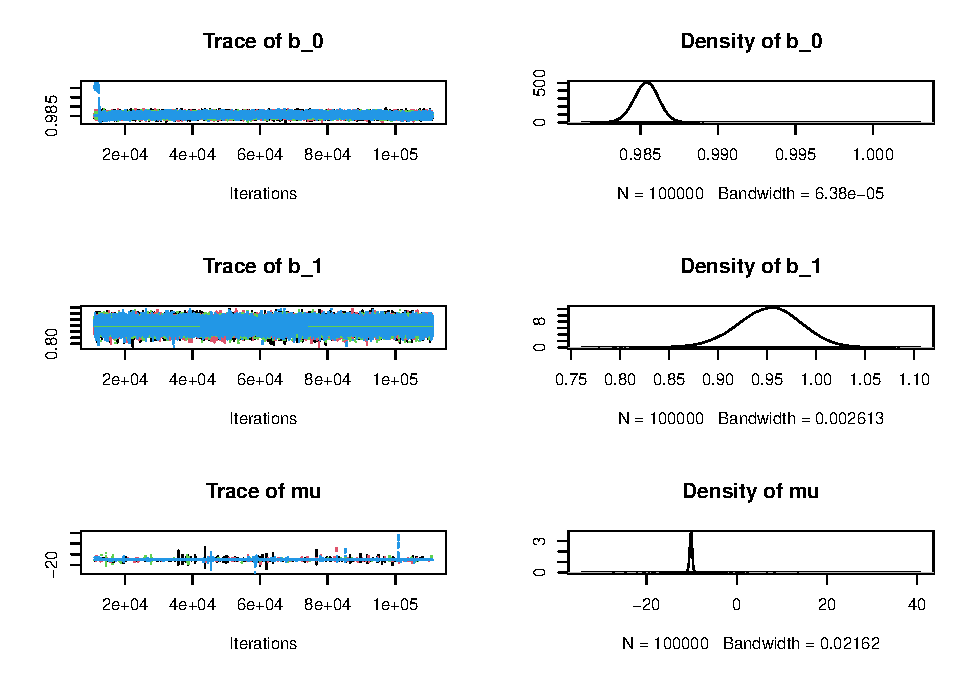
\includegraphics{assignment-1_files/figure-latex/unnamed-chunk-7-1.pdf}
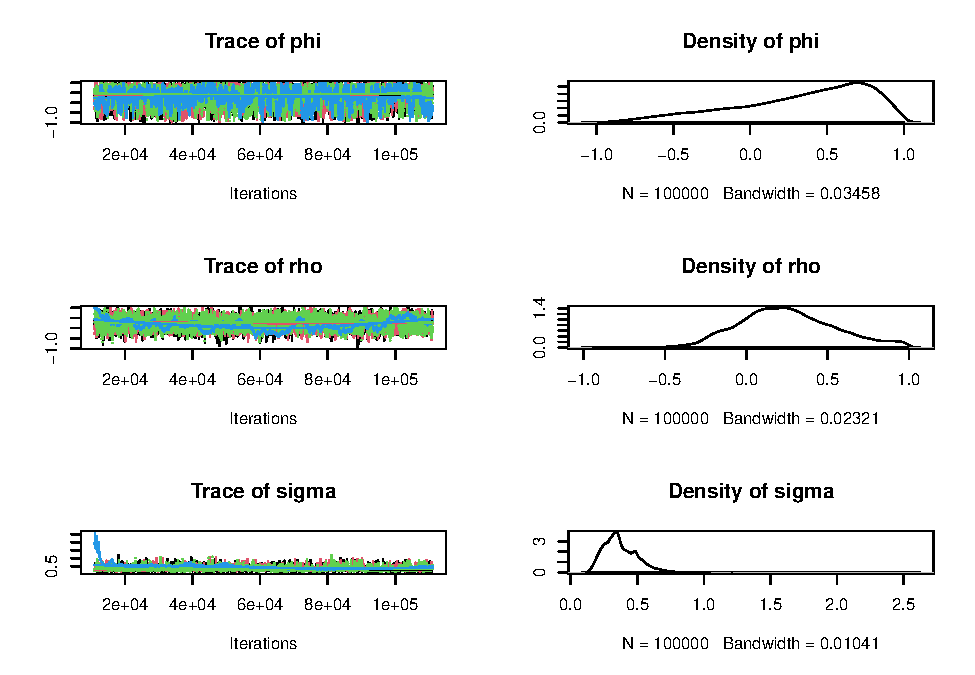
\includegraphics{assignment-1_files/figure-latex/unnamed-chunk-7-2.pdf}

There seems to be some problem with the mixing, my implementation looks
unstable, I tried running it a few times without changing the priors and
the results vary.

\begin{Shaded}
\begin{Highlighting}[]
\DocumentationTok{\#\# Setting 3x2 plots displayed next to each other}
\FunctionTok{par}\NormalTok{(}\AttributeTok{mfrow=}\FunctionTok{c}\NormalTok{(}\DecValTok{3}\NormalTok{,}\DecValTok{2}\NormalTok{))}

\DocumentationTok{\#\# Gelman statistic and plots}

\FunctionTok{gelman.diag}\NormalTok{(samples\_q1a)}
\end{Highlighting}
\end{Shaded}

\begin{verbatim}
## Potential scale reduction factors:
## 
##       Point est. Upper C.I.
## b_0         1.00       1.00
## b_1         1.00       1.00
## mu          1.05       1.05
## phi         1.00       1.01
## rho         1.00       1.01
## sigma       1.00       1.00
## 
## Multivariate psrf
## 
## 1
\end{verbatim}

\begin{Shaded}
\begin{Highlighting}[]
\FunctionTok{gelman.plot}\NormalTok{(samples\_q1a)}
\end{Highlighting}
\end{Shaded}

\includegraphics{assignment-1_files/figure-latex/unnamed-chunk-8-1.pdf}

The Gelman statistic is close to 1 for some of the hyperparameters but
not all of them which suggests that there is a sign of non-convergence.

\begin{Shaded}
\begin{Highlighting}[]
\DocumentationTok{\#\# Setting 3x2 plots displayed next to each other}
\FunctionTok{par}\NormalTok{(}\AttributeTok{mfrow=}\FunctionTok{c}\NormalTok{(}\DecValTok{3}\NormalTok{,}\DecValTok{2}\NormalTok{))}
\FunctionTok{par}\NormalTok{(}\AttributeTok{mar=}\FunctionTok{c}\NormalTok{(}\DecValTok{1}\NormalTok{,}\DecValTok{1}\NormalTok{,}\DecValTok{1}\NormalTok{,}\DecValTok{1}\NormalTok{))}

\DocumentationTok{\#\# Autocorrelation plots}
\FunctionTok{acf}\NormalTok{(samples\_q1a[[}\DecValTok{1}\NormalTok{]][,}\StringTok{"b\_0"}\NormalTok{])}
\FunctionTok{acf}\NormalTok{(samples\_q1a[[}\DecValTok{1}\NormalTok{]][,}\StringTok{"b\_1"}\NormalTok{])}
\FunctionTok{acf}\NormalTok{(samples\_q1a[[}\DecValTok{1}\NormalTok{]][,}\StringTok{"rho"}\NormalTok{])}
\FunctionTok{acf}\NormalTok{(samples\_q1a[[}\DecValTok{1}\NormalTok{]][,}\StringTok{"mu"}\NormalTok{])}
\FunctionTok{acf}\NormalTok{(samples\_q1a[[}\DecValTok{1}\NormalTok{]][,}\StringTok{"sigma"}\NormalTok{])}
\FunctionTok{acf}\NormalTok{(samples\_q1a[[}\DecValTok{1}\NormalTok{]][,}\StringTok{"phi"}\NormalTok{])}
\end{Highlighting}
\end{Shaded}

\includegraphics{assignment-1_files/figure-latex/unnamed-chunk-9-1.pdf}

\begin{Shaded}
\begin{Highlighting}[]
\DocumentationTok{\#\# Effective sample sizes for the parameters of interest }
\FunctionTok{effectiveSize}\NormalTok{(samples\_q1a)}
\end{Highlighting}
\end{Shaded}

\begin{verbatim}
##       b_0       b_1        mu       phi       rho     sigma 
## 18482.524 31529.095  9230.757  1778.958  2247.195  2946.127
\end{verbatim}

\textbf{Explanation}: Every prior was chosen to be non-informative,
since we don't possess any expert knowledge on the problem. Furthermore
we have taken into account the support of each parameter in the choice
of the prior. More specifically, b0,b1,mu are not constrained to a
specific interval, so we have chosen a normal prior with zero mean and
large variance to express our uncertainty, rho and phi are constrained
quantities so we have chosen a uniform prior over the interval (-1,1)
(for phi it is a uniform over (-0.99999,0.99999) because the original
interval is open), finally for sigma we have defined a prior indirectly
through tau in order to match JAGS definitions, a gamma prior was chosen
with parameters (0.1,0.1) to express our uncertainty with smaller values
of precision being more probable. For convergence diagnostics, we have
chosen to present the Gelman statistic and plots (which optimally should
be around 1), autocorrelation plots and effective sample sizes for all
parameters. In order to improve convergence we use centering and change
the step size. At this point, i would like to provide two additional
notes, I tried a few other non-informative priors e.g.~uniform priors
for mu and sigma and there seems to be some sensitivity to the choice of
priors, which looks reasonable considering the fact we only have 65
observed values. Finally, I tried a lot of alternative approaches to
implement this model and none of them seemed to work in a satisfactory
manner, for the implementation I have presented above the idea is that
since \$\$

\begin{aligned} 

(\epsilon_t,\eta_t)&\sim N\left(0, \Sigma_{\rho}\right)\quad \text{ for } \quad \Sigma_{\rho}=\left(\begin{matrix}1 & \rho\\ \rho & 1\end{matrix}\right)

\end{aligned}

we can prove that

\begin{aligned}

\eta_t&\sim N(0,1)\\ \epsilon_t|\eta_t&\sim N(\rho \eta_t ,(1-\rho)^2)

\end{aligned}

therefore we can try sampling \$\eta\_t\$. Some relevant here papers are
BUGS for a Bayesian analysis of stochastic volatility models , Meyer \&
Yu (2000),

Mean Correction and Higher Order Moments for a Stochastic Volatility
Model with Correlated Errors, Mukhoti \& Ranjan (2016) (I think my
implementation is not entirely correct, I am giving those resources here
as an indication of my thought process).

\textbf{b){[}10 marks{]} In practice, one often encounters outliers in
exchange rates. These can be sometimes modeled by assuming Student's t
distribution in the observation errors (i.e.} \(\epsilon_t\)).
\textbf{The robust leveraged SV model can be expressed as}

\(\begin{aligned} y_t&=\beta_0+\beta_1 y_{t-1}+\exp(h_t/2)\epsilon_t \quad \text{for}\quad 1\le t\le T,\\ h_{t+1}&=\mu+\phi(h_t-\mu)+\sigma \eta_t\quad \text{for} \quad 0\le t\le T, \quad h_0\sim N(\mu, \sigma^2/(1-\phi^2)),\\ \eta_t&\sim N(0,1)\\ \epsilon_t|\eta_t&\sim t_{\nu}(\rho \eta_t ,1). \end{aligned}\)

\textbf{Here} \(\nu\) \textbf{is the degrees of freedom parameter
(unknown).}

\textbf{Implement this model in JAGS or Stan on the first 3 months of
USD/EUR data from the dataset.}

\textbf{Explain how did you choose priors for all parameters. Explain
how did you take into account the days without observation in your
model.}

\textbf{Fit the model, do convergence diagnostics, print out the summary
of the results, and discuss them.}

\textbf{Make sure that the Effective Sample Size is at least 1000 for
all 6 hyperparameters (you need to choose burn-in and number of steps
appropriately for this).}

\begin{Shaded}
\begin{Highlighting}[]
\DocumentationTok{\#\# We define the model as in q1a, here we have an extra hyperparameter nu, for }
\DocumentationTok{\#\# we define a chi{-}squared prior}

\NormalTok{model\_string\_q1b }\OtherTok{\textless{}{-}} \StringTok{" model\{}
\StringTok{  }
\StringTok{  \#\# Priors for hyperparameters}
\StringTok{  }
\StringTok{  mu \textasciitilde{} dnorm(0, 1e{-}5)}
\StringTok{  phi \textasciitilde{} dunif({-}0.99999, 0.99999)}
\StringTok{  rho \textasciitilde{} dunif({-}1, 1)}
\StringTok{  }
\StringTok{  tau \textasciitilde{} dgamma(0.1, 0.1)}
\StringTok{  sigma2 \textless{}{-} 1/tau}
\StringTok{  sigma \textless{}{-} sqrt(sigma2)}
\StringTok{  }
\StringTok{  b\_0 \textasciitilde{} dnorm(0, 1e{-}4)}
\StringTok{  b\_1 \textasciitilde{} dnorm(0, 1e{-}4)}
\StringTok{  }
\StringTok{  nu \textasciitilde{} dgamma(0.1,0.1)}
\StringTok{  }
\StringTok{  \#\# Priors for initialiasations}
\StringTok{  }
\StringTok{  eta[1] \textasciitilde{} dnorm(0,1)}
\StringTok{  }
\StringTok{  \#\# h[1]}
\StringTok{  h\_0 \textasciitilde{} dnorm(mu, tau1)}
\StringTok{  tau1 \textless{}{-} (1{-}phi**2)/sigma2}
\StringTok{  mu\_h[1] \textless{}{-} mu + phi*(h\_0{-}mu) + sigma*eta[1]}
\StringTok{  h[1] \textasciitilde{} dnorm(mu\_h[1],tau)}
\StringTok{  }
\StringTok{  \#\# y[1]}
\StringTok{  y\_0 \textasciitilde{} dnorm(0,1e{-}5)}
\StringTok{  mu\_y[1] \textless{}{-} b\_0 + b\_1*(y\_0{-}meanY) + exp(h[1]/2)*rho*eta[1]}
\StringTok{  y[1] \textasciitilde{} dt(mu\_y[1],(exp({-}h[1])/(1{-}rho**2)),nu)}
\StringTok{  y\_rep[1] \textasciitilde{} dt(mu\_y[1],(exp({-}h[1])/(1{-}rho**2)),nu)}
\StringTok{  }
\StringTok{  \#\# Likelihood}
\StringTok{  }
\StringTok{  for (t in 2:n)\{}
\StringTok{  }
\StringTok{    eta[t] \textasciitilde{} dnorm(0,1)}
\StringTok{    }
\StringTok{    \#\# Following workshop 1 we will use centering (i.e. subtracting the mean)}
\StringTok{    \#\# we do this to help with convergence }
\StringTok{    }
\StringTok{    mu\_y[t] \textless{}{-} b\_0 + b\_1*(y[t{-}1]{-}meanY) + exp(h[t]/2)*rho*eta[t]}
\StringTok{    }
\StringTok{    y[t] \textasciitilde{} dt(mu\_y[t], (exp({-}h[t])/(1{-}rho**2)),nu)}
\StringTok{    }
\StringTok{    \#\# Replicates used for posterior predictive checks in a later question}
\StringTok{    y\_rep[t]  \textasciitilde{} dt(mu\_y[t], (exp({-}h[t])/(1{-}rho**2)),nu)}
\StringTok{    }
\StringTok{    mu\_h[t] \textless{}{-} mu + phi*(h[t{-}1] {-} mu) + sigma*eta[t{-}1]}
\StringTok{    h[t] \textasciitilde{} dnorm(mu\_h[t], tau)}
\StringTok{  \}}
\StringTok{  }
\StringTok{  }
\StringTok{  }
\StringTok{\}"}
\end{Highlighting}
\end{Shaded}

\begin{Shaded}
\begin{Highlighting}[]
\DocumentationTok{\#\# compiling model the model using JAGS}
\NormalTok{model\_q1b }\OtherTok{\textless{}{-}} \FunctionTok{jags.model}\NormalTok{(}\FunctionTok{textConnection}\NormalTok{(model\_string\_q1b), }
                      \AttributeTok{data =} \FunctionTok{list}\NormalTok{(}\AttributeTok{y =}\NormalTok{ y\_usd, }\AttributeTok{meanY =}\NormalTok{ meanY,  }\AttributeTok{n =}\NormalTok{ n), }\AttributeTok{n.chains =} \DecValTok{4}\NormalTok{)}
\end{Highlighting}
\end{Shaded}

\begin{verbatim}
## Compiling model graph
##    Resolving undeclared variables
##    Allocating nodes
## Graph information:
##    Observed stochastic nodes: 65
##    Unobserved stochastic nodes: 308
##    Total graph size: 1567
## 
## Initializing model
\end{verbatim}

\begin{Shaded}
\begin{Highlighting}[]
\DocumentationTok{\#\# Choosing burn{-}in }
\FunctionTok{update}\NormalTok{(model\_q1b,}\DecValTok{10000}\NormalTok{,}\AttributeTok{progress.bar=}\StringTok{"none"}\NormalTok{)}


\DocumentationTok{\#\# Collecting sample from the model}
\DocumentationTok{\#\# 100k iterations with 50 thinning }
\NormalTok{samples\_q1b }\OtherTok{\textless{}{-}} \FunctionTok{coda.samples}\NormalTok{(model\_q1b, }\AttributeTok{variable.names =} \FunctionTok{c}\NormalTok{(}\StringTok{"b\_0"}\NormalTok{, }\StringTok{"b\_1"}\NormalTok{, }\StringTok{"mu"}\NormalTok{, }\StringTok{"phi"}\NormalTok{, }\StringTok{"sigma"}\NormalTok{, }\StringTok{"rho"}\NormalTok{,}\StringTok{"nu"}\NormalTok{), }\AttributeTok{n.iter =} \DecValTok{100000}\NormalTok{, }\AttributeTok{progress.bar=}\StringTok{"none"}\NormalTok{,}\AttributeTok{n.thin=}\DecValTok{50}\NormalTok{,}\AttributeTok{stepsize=}\NormalTok{stepsize)}
\end{Highlighting}
\end{Shaded}

Run time :: approximately 11 minutes

\begin{Shaded}
\begin{Highlighting}[]
\DocumentationTok{\#\# summary}
\FunctionTok{summary}\NormalTok{(samples\_q1b)}
\end{Highlighting}
\end{Shaded}

\begin{verbatim}
## 
## Iterations = 11001:111000
## Thinning interval = 1 
## Number of chains = 4 
## Sample size per chain = 1e+05 
## 
## 1. Empirical mean and standard deviation for each variable,
##    plus standard error of the mean:
## 
##           Mean        SD  Naive SE Time-series SE
## b_0     0.9857 0.0007345 1.161e-06      4.630e-06
## b_1     0.9532 0.0318425 5.035e-05      1.883e-04
## mu    -10.2405 0.4245088 6.712e-04      4.531e-03
## nu      9.3497 7.4003243 1.170e-02      5.369e-02
## phi     0.3040 0.4460979 7.053e-04      1.002e-02
## rho     0.2731 0.5661694 8.952e-04      1.531e-02
## sigma   0.3695 0.1309668 2.071e-04      2.394e-03
## 
## 2. Quantiles for each variable:
## 
##           2.5%        25%      50%      75%   97.5%
## b_0     0.9843   0.985237   0.9857   0.9862  0.9872
## b_1     0.8893   0.932314   0.9537   0.9746  1.0146
## mu    -10.8854 -10.433759 -10.2372 -10.0462 -9.6271
## nu      1.8977   4.397075   7.1426  11.8794 29.3991
## phi    -0.6601  -0.006689   0.3858   0.6722  0.9305
## rho    -0.9015  -0.151283   0.4148   0.7612  0.9812
## sigma   0.1777   0.274451   0.3484   0.4414  0.6826
\end{verbatim}

We observe that the summary of the results is very similar with question
(a).

\begin{Shaded}
\begin{Highlighting}[]
\FunctionTok{par}\NormalTok{(}\AttributeTok{mar=}\FunctionTok{c}\NormalTok{(}\DecValTok{1}\NormalTok{,}\DecValTok{1}\NormalTok{,}\DecValTok{1}\NormalTok{,}\DecValTok{1}\NormalTok{))}
\DocumentationTok{\#\# Sample plots}
\FunctionTok{plot}\NormalTok{(samples\_q1b)}
\end{Highlighting}
\end{Shaded}

\includegraphics{assignment-1_files/figure-latex/unnamed-chunk-14-1.pdf}
\includegraphics{assignment-1_files/figure-latex/unnamed-chunk-14-2.pdf}

\begin{Shaded}
\begin{Highlighting}[]
\DocumentationTok{\#\# Setting 3x2 plots displayed next to each other}
\FunctionTok{par}\NormalTok{(}\AttributeTok{mfrow=}\FunctionTok{c}\NormalTok{(}\DecValTok{3}\NormalTok{,}\DecValTok{2}\NormalTok{))}
\FunctionTok{par}\NormalTok{(}\AttributeTok{mar=}\FunctionTok{c}\NormalTok{(}\DecValTok{1}\NormalTok{,}\DecValTok{1}\NormalTok{,}\DecValTok{1}\NormalTok{,}\DecValTok{1}\NormalTok{))}

\DocumentationTok{\#\# Autocorrelation plots}
\FunctionTok{acf}\NormalTok{(samples\_q1b[[}\DecValTok{1}\NormalTok{]][,}\StringTok{"b\_0"}\NormalTok{])}
\FunctionTok{acf}\NormalTok{(samples\_q1b[[}\DecValTok{1}\NormalTok{]][,}\StringTok{"b\_1"}\NormalTok{])}
\FunctionTok{acf}\NormalTok{(samples\_q1b[[}\DecValTok{1}\NormalTok{]][,}\StringTok{"rho"}\NormalTok{])}
\FunctionTok{acf}\NormalTok{(samples\_q1b[[}\DecValTok{1}\NormalTok{]][,}\StringTok{"mu"}\NormalTok{])}
\FunctionTok{acf}\NormalTok{(samples\_q1b[[}\DecValTok{1}\NormalTok{]][,}\StringTok{"sigma"}\NormalTok{])}
\FunctionTok{acf}\NormalTok{(samples\_q1b[[}\DecValTok{1}\NormalTok{]][,}\StringTok{"phi"}\NormalTok{])}
\end{Highlighting}
\end{Shaded}

\includegraphics{assignment-1_files/figure-latex/unnamed-chunk-15-1.pdf}

\begin{Shaded}
\begin{Highlighting}[]
\FunctionTok{acf}\NormalTok{(samples\_q1b[[}\DecValTok{1}\NormalTok{]][,}\StringTok{"nu"}\NormalTok{])}
\end{Highlighting}
\end{Shaded}

\includegraphics{assignment-1_files/figure-latex/unnamed-chunk-15-2.pdf}

Again high autocorrelation seems to persist we see that in the sample
sizes as well.

\begin{Shaded}
\begin{Highlighting}[]
\DocumentationTok{\#\# Effective sample sizes for the parameters of interest }
\FunctionTok{effectiveSize}\NormalTok{(samples\_q1b)}
\end{Highlighting}
\end{Shaded}

\begin{verbatim}
##       b_0       b_1        mu        nu       phi       rho     sigma 
## 25335.325 28637.849  8756.752 19049.232  1988.425  1368.480  3029.796
\end{verbatim}

\textbf{Explanation}: The choice of priors here is the same as in
question 1. Additionally, for the degrees of freedom we have chosen a
gamma prior, following what we did for the precision. The idea for the
implementation is the same as in question 1, however here we use a t
likelihood for the observations.

\textbf{c){[}10 marks{]}}

\textbf{Perform posterior predictive checks on both models a) and b).
Explain how did you choose the test functions.}

\begin{Shaded}
\begin{Highlighting}[]
\DocumentationTok{\#\# we shall use the replicates we declared in the previous questions}

\DocumentationTok{\#\# For model\_q1a}
\NormalTok{y\_rep\_q1a }\OtherTok{=} \FunctionTok{coda.samples}\NormalTok{(model\_q1a, }\AttributeTok{variable.names=}\FunctionTok{c}\NormalTok{(}\StringTok{"y\_rep"}\NormalTok{),}\AttributeTok{n.iter=}\DecValTok{20000}\NormalTok{,}\AttributeTok{n.thin=}\DecValTok{10}\NormalTok{)}

\DocumentationTok{\#\# For model\_q1b}
\NormalTok{y\_rep\_q1b }\OtherTok{=} \FunctionTok{coda.samples}\NormalTok{(model\_q1b, }\AttributeTok{variable.names=}\FunctionTok{c}\NormalTok{(}\StringTok{"y\_rep"}\NormalTok{),}\AttributeTok{n.iter=}\DecValTok{20000}\NormalTok{,}\AttributeTok{n.thin=}\DecValTok{10}\NormalTok{)}
\end{Highlighting}
\end{Shaded}

Run time :: approximately 3 minutes

\begin{Shaded}
\begin{Highlighting}[]
\DocumentationTok{\#\# For model\_q1a}

\NormalTok{ind\_yrep\_not\_NA }\OtherTok{=} \FunctionTok{which}\NormalTok{(}\SpecialCharTok{!}\FunctionTok{is.na}\NormalTok{(y\_usd))}
\NormalTok{y\_not\_NA }\OtherTok{=}\NormalTok{ y\_usd[}\SpecialCharTok{!}\FunctionTok{is.na}\NormalTok{(y\_usd)]}


\NormalTok{yrep\_q1a\_samples}\OtherTok{=}\FunctionTok{data.frame}\NormalTok{(}\FunctionTok{rbind}\NormalTok{(y\_rep\_q1a[[}\DecValTok{1}\NormalTok{]][,ind\_yrep\_not\_NA],y\_rep\_q1a[[}\DecValTok{2}\NormalTok{]][,ind\_yrep\_not\_NA],}
\NormalTok{                              y\_rep\_q1a[[}\DecValTok{3}\NormalTok{]][,ind\_yrep\_not\_NA],y\_rep\_q1a[[}\DecValTok{4}\NormalTok{]][,ind\_yrep\_not\_NA]))}
\NormalTok{yrep\_q1a\_samples.min}\OtherTok{=}\FunctionTok{apply}\NormalTok{(yrep\_q1a\_samples,}\AttributeTok{MARGIN=}\DecValTok{1}\NormalTok{, }\AttributeTok{FUN=}\NormalTok{min)}
\NormalTok{yrep\_q1a\_samples.max}\OtherTok{=}\FunctionTok{apply}\NormalTok{(yrep\_q1a\_samples,}\AttributeTok{MARGIN=}\DecValTok{1}\NormalTok{, }\AttributeTok{FUN=}\NormalTok{max)}
\NormalTok{yrep\_q1a\_samples.median}\OtherTok{=}\FunctionTok{apply}\NormalTok{(yrep\_q1a\_samples,}\AttributeTok{MARGIN=}\DecValTok{1}\NormalTok{, }\AttributeTok{FUN=}\NormalTok{median)}

\FunctionTok{par}\NormalTok{(}\AttributeTok{mfrow=}\FunctionTok{c}\NormalTok{(}\DecValTok{3}\NormalTok{,}\DecValTok{2}\NormalTok{))}
\FunctionTok{par}\NormalTok{(}\AttributeTok{mar=}\FunctionTok{c}\NormalTok{(}\DecValTok{1}\NormalTok{,}\DecValTok{1}\NormalTok{,}\DecValTok{1}\NormalTok{,}\DecValTok{1}\NormalTok{))}
\FunctionTok{hist}\NormalTok{(yrep\_q1a\_samples.min,}\AttributeTok{col=}\StringTok{"gray40"}\NormalTok{,}\AttributeTok{main=}\StringTok{"Predictive distribution for min"}\NormalTok{)}
\FunctionTok{abline}\NormalTok{(}\AttributeTok{v=}\FunctionTok{min}\NormalTok{(y\_not\_NA),}\AttributeTok{col=}\StringTok{"red"}\NormalTok{,}\AttributeTok{lwd=}\DecValTok{2}\NormalTok{)}
\FunctionTok{hist}\NormalTok{(yrep\_q1a\_samples.max,}\AttributeTok{col=}\StringTok{"gray40"}\NormalTok{,}\AttributeTok{main=}\StringTok{"Predictive distribution for max"}\NormalTok{)}
\FunctionTok{abline}\NormalTok{(}\AttributeTok{v=}\FunctionTok{max}\NormalTok{(y\_not\_NA),}\AttributeTok{col=}\StringTok{"red"}\NormalTok{,}\AttributeTok{lwd=}\DecValTok{2}\NormalTok{)}
\FunctionTok{hist}\NormalTok{(yrep\_q1a\_samples.median,}\AttributeTok{col=}\StringTok{"gray40"}\NormalTok{,}\AttributeTok{main=}\StringTok{"Predictive distribution for median"}\NormalTok{)}
\FunctionTok{abline}\NormalTok{(}\AttributeTok{v=}\FunctionTok{median}\NormalTok{(y\_not\_NA),}\AttributeTok{col=}\StringTok{"red"}\NormalTok{,}\AttributeTok{lwd=}\DecValTok{2}\NormalTok{)}
\end{Highlighting}
\end{Shaded}

\includegraphics{assignment-1_files/figure-latex/unnamed-chunk-18-1.pdf}

\begin{Shaded}
\begin{Highlighting}[]
\DocumentationTok{\#\# For model\_q1b}


\NormalTok{yrep\_q1b\_samples}\OtherTok{=}\FunctionTok{data.frame}\NormalTok{(}\FunctionTok{rbind}\NormalTok{(y\_rep\_q1b[[}\DecValTok{1}\NormalTok{]][,ind\_yrep\_not\_NA],y\_rep\_q1b[[}\DecValTok{2}\NormalTok{]][,ind\_yrep\_not\_NA],}
\NormalTok{                              y\_rep\_q1b[[}\DecValTok{3}\NormalTok{]][,ind\_yrep\_not\_NA],y\_rep\_q1b[[}\DecValTok{4}\NormalTok{]][,ind\_yrep\_not\_NA]))}
\NormalTok{yrep\_q1b\_samples.min}\OtherTok{=}\FunctionTok{apply}\NormalTok{(yrep\_q1b\_samples,}\AttributeTok{MARGIN=}\DecValTok{1}\NormalTok{, }\AttributeTok{FUN=}\NormalTok{min)}
\NormalTok{yrep\_q1b\_samples.max}\OtherTok{=}\FunctionTok{apply}\NormalTok{(yrep\_q1b\_samples,}\AttributeTok{MARGIN=}\DecValTok{1}\NormalTok{, }\AttributeTok{FUN=}\NormalTok{max)}
\NormalTok{yrep\_q1b\_samples.median}\OtherTok{=}\FunctionTok{apply}\NormalTok{(yrep\_q1b\_samples,}\AttributeTok{MARGIN=}\DecValTok{1}\NormalTok{, }\AttributeTok{FUN=}\NormalTok{median)}

\FunctionTok{par}\NormalTok{(}\AttributeTok{mfrow=}\FunctionTok{c}\NormalTok{(}\DecValTok{3}\NormalTok{,}\DecValTok{2}\NormalTok{))}
\FunctionTok{par}\NormalTok{(}\AttributeTok{mar=}\FunctionTok{c}\NormalTok{(}\DecValTok{1}\NormalTok{,}\DecValTok{1}\NormalTok{,}\DecValTok{1}\NormalTok{,}\DecValTok{1}\NormalTok{))}
\FunctionTok{hist}\NormalTok{(yrep\_q1b\_samples.min,}\AttributeTok{col=}\StringTok{"gray40"}\NormalTok{,}\AttributeTok{main=}\StringTok{"Predictive distribution for min"}\NormalTok{)}
\FunctionTok{abline}\NormalTok{(}\AttributeTok{v=}\FunctionTok{min}\NormalTok{(y\_not\_NA),}\AttributeTok{col=}\StringTok{"red"}\NormalTok{,}\AttributeTok{lwd=}\DecValTok{2}\NormalTok{)}
\FunctionTok{hist}\NormalTok{(yrep\_q1b\_samples.max,}\AttributeTok{col=}\StringTok{"gray40"}\NormalTok{,}\AttributeTok{main=}\StringTok{"Predictive distribution for max"}\NormalTok{)}
\FunctionTok{abline}\NormalTok{(}\AttributeTok{v=}\FunctionTok{max}\NormalTok{(y\_not\_NA),}\AttributeTok{col=}\StringTok{"red"}\NormalTok{,}\AttributeTok{lwd=}\DecValTok{2}\NormalTok{)}
\FunctionTok{hist}\NormalTok{(yrep\_q1b\_samples.median,}\AttributeTok{col=}\StringTok{"gray40"}\NormalTok{,}\AttributeTok{main=}\StringTok{"Predictive distribution for median"}\NormalTok{)}
\FunctionTok{abline}\NormalTok{(}\AttributeTok{v=}\FunctionTok{median}\NormalTok{(y\_not\_NA),}\AttributeTok{col=}\StringTok{"red"}\NormalTok{,}\AttributeTok{lwd=}\DecValTok{2}\NormalTok{)}
\end{Highlighting}
\end{Shaded}

\includegraphics{assignment-1_files/figure-latex/unnamed-chunk-19-1.pdf}

\textbf{Perform posterior predictive checks on both models a) and b).
Explain how did you choose the test functions.}

\textbf{Discuss the results.} \textbf{Explanation}: We have created
replicates by including them in the model. We obtain samples from the
replicates by coda.samples, with y.rep included in variable.names. We
have pruned out the observations with NA values from the replicates (as
they would distort the results), and compared the values of the
functions min, max, median on the data with the histograms of the
replicates. We have chosen min,max,median based on orthogonality with
model parameters (slides Lecture 1). As we can see the posterior
predictive checks do not detect any problems with either one of the two
models.

\textbf{d){[}10 marks{]}}

\textbf{Based on your models a) and b), plot the posterior predictive
densities of the USD/EUR rate on the dates 2000-04-03, 2020-04-04 and
2020-04-05 (the next 3 days after the period considered). Compute the
posterior means and 95\% credible intervals. Discuss the results.}

\begin{Shaded}
\begin{Highlighting}[]
\DocumentationTok{\#\# I answer on the premise that you mean 2000{-}04{-}03, 2000{-}04{-}04 and}
\DocumentationTok{\#\# 2000{-}04{-}05}

\DocumentationTok{\#\# We create a new data vector with NA for these dates, just like we did in part (a)}

\DocumentationTok{\#\# Extracting usd\_eur forex pair}
\NormalTok{usd\_eur }\OtherTok{\textless{}{-}}\NormalTok{ exrates}\SpecialCharTok{$}\NormalTok{USD}

\DocumentationTok{\#\# Extracting dates}
\NormalTok{dates\_d }\OtherTok{\textless{}{-}}\NormalTok{ exrates}\SpecialCharTok{$}\NormalTok{date}

\NormalTok{pos1d }\OtherTok{\textless{}{-}} \FunctionTok{which}\NormalTok{(dates}\SpecialCharTok{==}\StringTok{\textquotesingle{}2000{-}01{-}03\textquotesingle{}}\NormalTok{)}
\NormalTok{pos2d }\OtherTok{\textless{}{-}} \FunctionTok{which}\NormalTok{(dates}\SpecialCharTok{==}\StringTok{\textquotesingle{}2000{-}03{-}31\textquotesingle{}}\NormalTok{)}

\DocumentationTok{\#\# Generating the full sequence of dates}
\NormalTok{full\_dates\_d }\OtherTok{\textless{}{-}} \FunctionTok{seq}\NormalTok{(}\FunctionTok{as.Date}\NormalTok{(}\StringTok{\textquotesingle{}2000{-}01{-}03\textquotesingle{}}\NormalTok{), }\FunctionTok{as.Date}\NormalTok{(}\StringTok{\textquotesingle{}2000{-}04{-}05\textquotesingle{}}\NormalTok{), }\AttributeTok{by=}\StringTok{"days"}\NormalTok{)}

\DocumentationTok{\#\# Keeping only the dates of interest in the initial vector}
\NormalTok{dates\_d }\OtherTok{\textless{}{-}}\NormalTok{ dates\_d[pos1}\SpecialCharTok{:}\NormalTok{pos2]}

\DocumentationTok{\#\# Obtaining the index of observed values}
\NormalTok{ind }\OtherTok{\textless{}{-}} \FunctionTok{c}\NormalTok{()}

\ControlFlowTok{for}\NormalTok{(i }\ControlFlowTok{in} \FunctionTok{seq}\NormalTok{(}\DecValTok{1}\SpecialCharTok{:}\FunctionTok{length}\NormalTok{(dates)))\{}
  
\NormalTok{  ind[i] }\OtherTok{\textless{}{-}} \FunctionTok{which}\NormalTok{(dates[i]}\SpecialCharTok{==}\NormalTok{full\_dates\_d)}
  
\NormalTok{\}}

\DocumentationTok{\#\# Final vector of observations with NA values for weekends and holidays}

\NormalTok{y\_usd\_new }\OtherTok{\textless{}{-}} \FunctionTok{rep}\NormalTok{(}\ConstantTok{NA}\NormalTok{,}\FunctionTok{length}\NormalTok{(full\_dates\_d))}
\NormalTok{usd\_eur }\OtherTok{\textless{}{-}}\NormalTok{ usd\_eur[pos1}\SpecialCharTok{:}\NormalTok{pos2]}
\NormalTok{y\_usd\_new[ind] }\OtherTok{\textless{}{-}}\NormalTok{ usd\_eur}



\DocumentationTok{\#\# Total number of days, needed for model compilation}
\NormalTok{n\_d }\OtherTok{\textless{}{-}} \FunctionTok{length}\NormalTok{(y\_usd\_new)}

\DocumentationTok{\#\# Mean of the observations, excluding NA values}
\DocumentationTok{\#\# We will use the mean for centering our observations to help convergence}
\NormalTok{meanY }\OtherTok{\textless{}{-}} \FunctionTok{mean}\NormalTok{(usd\_eur)}

\NormalTok{model\_q1a\_d }\OtherTok{\textless{}{-}} \FunctionTok{jags.model}\NormalTok{(}\FunctionTok{textConnection}\NormalTok{(model\_string\_q1a), }
                      \AttributeTok{data =} \FunctionTok{list}\NormalTok{(}\AttributeTok{y =}\NormalTok{ y\_usd\_new, }\AttributeTok{meanY =}\NormalTok{ meanY,  }\AttributeTok{n =}\NormalTok{ n\_d), }\AttributeTok{n.chains =} \DecValTok{4}\NormalTok{)}
\end{Highlighting}
\end{Shaded}

\begin{verbatim}
## Compiling model graph
##    Resolving undeclared variables
##    Allocating nodes
## Graph information:
##    Observed stochastic nodes: 65
##    Unobserved stochastic nodes: 319
##    Total graph size: 1897
## 
## Initializing model
\end{verbatim}

\begin{Shaded}
\begin{Highlighting}[]
\NormalTok{ypost1\_replicates }\OtherTok{\textless{}{-}} \FunctionTok{coda.samples}\NormalTok{(model\_q1a\_d,}\AttributeTok{variable.names=}\FunctionTok{c}\NormalTok{(}\StringTok{"y\_rep"}\NormalTok{),}\AttributeTok{n.iter=}\DecValTok{20000}\NormalTok{, }\AttributeTok{progress.bar=}\StringTok{"none"}\NormalTok{, }\AttributeTok{n.thin=}\DecValTok{5}\NormalTok{) }

\NormalTok{ypost1\_mat }\OtherTok{\textless{}{-}} \FunctionTok{as.matrix}\NormalTok{(ypost1\_replicates)}
\NormalTok{ypost1 }\OtherTok{\textless{}{-}} \FunctionTok{as.matrix}\NormalTok{(ypost1\_mat[,(}\FunctionTok{ncol}\NormalTok{(ypost1\_mat)}\SpecialCharTok{{-}}\DecValTok{2}\NormalTok{)}\SpecialCharTok{:}\FunctionTok{ncol}\NormalTok{(ypost1\_mat)])}

\NormalTok{post1\_mean }\OtherTok{\textless{}{-}} \FunctionTok{apply}\NormalTok{(ypost1, }\DecValTok{2}\NormalTok{, mean)}
\NormalTok{post1\_sd }\OtherTok{\textless{}{-}} \FunctionTok{apply}\NormalTok{(ypost1, }\DecValTok{2}\NormalTok{, sd)}

\DocumentationTok{\#\# Upper and lower limits}

\NormalTok{cred\_ul1 }\OtherTok{\textless{}{-}}\NormalTok{ post1\_mean[}\DecValTok{1}\NormalTok{] }\SpecialCharTok{+} \FloatTok{1.96} \SpecialCharTok{*}\NormalTok{ post1\_sd[}\DecValTok{1}\NormalTok{]}
\NormalTok{cred\_ll1 }\OtherTok{\textless{}{-}}\NormalTok{ post1\_mean[}\DecValTok{1}\NormalTok{] }\SpecialCharTok{{-}} \FloatTok{1.96} \SpecialCharTok{*}\NormalTok{ post1\_sd[}\DecValTok{1}\NormalTok{]}


\NormalTok{cred\_ul2 }\OtherTok{\textless{}{-}}\NormalTok{ post1\_mean[}\DecValTok{2}\NormalTok{] }\SpecialCharTok{+} \FloatTok{1.96} \SpecialCharTok{*}\NormalTok{ post1\_sd[}\DecValTok{2}\NormalTok{]}
\NormalTok{cred\_ll2 }\OtherTok{\textless{}{-}}\NormalTok{ post1\_mean[}\DecValTok{2}\NormalTok{] }\SpecialCharTok{{-}} \FloatTok{1.96} \SpecialCharTok{*}\NormalTok{ post1\_sd[}\DecValTok{2}\NormalTok{]}


\NormalTok{cred\_ul3 }\OtherTok{\textless{}{-}}\NormalTok{ post1\_mean[}\DecValTok{3}\NormalTok{] }\SpecialCharTok{+} \FloatTok{1.96} \SpecialCharTok{*}\NormalTok{ post1\_sd[}\DecValTok{3}\NormalTok{]}
\NormalTok{cred\_ll3 }\OtherTok{\textless{}{-}}\NormalTok{ post1\_mean[}\DecValTok{3}\NormalTok{] }\SpecialCharTok{{-}} \FloatTok{1.96} \SpecialCharTok{*}\NormalTok{ post1\_sd[}\DecValTok{3}\NormalTok{]}


\FunctionTok{plot}\NormalTok{(}\FunctionTok{density}\NormalTok{(ypost1[, }\DecValTok{1}\NormalTok{]), }\AttributeTok{main=}\StringTok{"95\% credible interval for 2000{-}04{-}03 "}\NormalTok{,}\AttributeTok{col=}\StringTok{\textquotesingle{}black\textquotesingle{}}\NormalTok{)}
\FunctionTok{points}\NormalTok{(y\_usd\_new[n\_d}\DecValTok{{-}2}\NormalTok{], }\DecValTok{0}\NormalTok{, }\AttributeTok{col =} \StringTok{"red"}\NormalTok{, }\AttributeTok{pch =} \DecValTok{19}\NormalTok{) }\DocumentationTok{\#\# True value}
\FunctionTok{abline}\NormalTok{(}\AttributeTok{v=}\FunctionTok{c}\NormalTok{(cred\_ul1, cred\_ll1),}\AttributeTok{col=}\StringTok{"red"}\NormalTok{,}\AttributeTok{lwd=}\DecValTok{2}\NormalTok{, }\AttributeTok{lty =} \DecValTok{2}\NormalTok{)}
\end{Highlighting}
\end{Shaded}

\includegraphics{assignment-1_files/figure-latex/unnamed-chunk-20-1.pdf}

\begin{Shaded}
\begin{Highlighting}[]
\FunctionTok{plot}\NormalTok{(}\FunctionTok{density}\NormalTok{(ypost1[, }\DecValTok{2}\NormalTok{]), }\AttributeTok{main=}\StringTok{"95\% credible interval for 2000{-}04{-}04 "}\NormalTok{, }\AttributeTok{col=}\StringTok{\textquotesingle{}black\textquotesingle{}}\NormalTok{)}
\FunctionTok{points}\NormalTok{(y\_usd\_new[n\_d}\DecValTok{{-}1}\NormalTok{], }\DecValTok{0}\NormalTok{, }\AttributeTok{col =} \StringTok{"red"}\NormalTok{, }\AttributeTok{pch =} \DecValTok{19}\NormalTok{) }\DocumentationTok{\#\# True value}
\FunctionTok{abline}\NormalTok{(}\AttributeTok{v=}\FunctionTok{c}\NormalTok{(cred\_ul2, cred\_ll2),}\AttributeTok{col=}\StringTok{"red"}\NormalTok{,}\AttributeTok{lwd=}\DecValTok{2}\NormalTok{, }\AttributeTok{lty =} \DecValTok{2}\NormalTok{)}
\end{Highlighting}
\end{Shaded}

\includegraphics{assignment-1_files/figure-latex/unnamed-chunk-21-1.pdf}

\begin{Shaded}
\begin{Highlighting}[]
\FunctionTok{plot}\NormalTok{(}\FunctionTok{density}\NormalTok{(ypost1[, }\DecValTok{3}\NormalTok{]), }\AttributeTok{main=}\StringTok{"95\% credible interval for 2000{-}04{-}05 "}\NormalTok{, }\AttributeTok{col=}\StringTok{"black"}\NormalTok{)}
\FunctionTok{points}\NormalTok{(y\_usd\_new[n\_d], }\DecValTok{0}\NormalTok{, }\AttributeTok{col =} \StringTok{"red"}\NormalTok{, }\AttributeTok{pch =} \DecValTok{19}\NormalTok{) }\DocumentationTok{\#\# True value}
\FunctionTok{abline}\NormalTok{(}\AttributeTok{v=}\FunctionTok{c}\NormalTok{(cred\_ul3, cred\_ll3),}\AttributeTok{col=}\StringTok{"red"}\NormalTok{,}\AttributeTok{lwd=}\DecValTok{2}\NormalTok{, }\AttributeTok{lty =} \DecValTok{2}\NormalTok{)}
\end{Highlighting}
\end{Shaded}

\includegraphics{assignment-1_files/figure-latex/unnamed-chunk-22-1.pdf}

\begin{Shaded}
\begin{Highlighting}[]
\DocumentationTok{\#\# For model q1b}
\NormalTok{model\_q1b\_d }\OtherTok{\textless{}{-}} \FunctionTok{jags.model}\NormalTok{(}\FunctionTok{textConnection}\NormalTok{(model\_string\_q1b), }
                      \AttributeTok{data =} \FunctionTok{list}\NormalTok{(}\AttributeTok{y =}\NormalTok{ y\_usd\_new, }\AttributeTok{meanY =}\NormalTok{ meanY,  }\AttributeTok{n =}\NormalTok{ n\_d), }\AttributeTok{n.chains =} \DecValTok{4}\NormalTok{)}
\end{Highlighting}
\end{Shaded}

\begin{verbatim}
## Compiling model graph
##    Resolving undeclared variables
##    Allocating nodes
## Graph information:
##    Observed stochastic nodes: 65
##    Unobserved stochastic nodes: 320
##    Total graph size: 1618
## 
## Initializing model
\end{verbatim}

\begin{Shaded}
\begin{Highlighting}[]
\NormalTok{ypost2\_replicates }\OtherTok{\textless{}{-}} \FunctionTok{coda.samples}\NormalTok{(model\_q1b\_d,}\AttributeTok{variable.names=}\FunctionTok{c}\NormalTok{(}\StringTok{"y\_rep"}\NormalTok{),}\AttributeTok{n.iter=}\DecValTok{10000}\NormalTok{, }\AttributeTok{progress.bar=}\StringTok{"none"}\NormalTok{, }\AttributeTok{n.thin=}\DecValTok{5}\NormalTok{) }

\NormalTok{ypost2\_mat }\OtherTok{\textless{}{-}} \FunctionTok{as.matrix}\NormalTok{(ypost2\_replicates)}
\NormalTok{ypost2 }\OtherTok{\textless{}{-}} \FunctionTok{as.matrix}\NormalTok{(ypost2\_mat[,(}\FunctionTok{ncol}\NormalTok{(ypost2\_mat)}\SpecialCharTok{{-}}\DecValTok{2}\NormalTok{)}\SpecialCharTok{:}\FunctionTok{ncol}\NormalTok{(ypost2\_mat)])}

\NormalTok{post2\_mean }\OtherTok{\textless{}{-}} \FunctionTok{apply}\NormalTok{(ypost2, }\DecValTok{2}\NormalTok{, mean)}
\NormalTok{post2\_sd }\OtherTok{\textless{}{-}} \FunctionTok{apply}\NormalTok{(ypost2, }\DecValTok{2}\NormalTok{, sd)}

\DocumentationTok{\#\# Upper and lower limits}

\NormalTok{cred2\_ul1 }\OtherTok{\textless{}{-}}\NormalTok{ post2\_mean[}\DecValTok{1}\NormalTok{] }\SpecialCharTok{+} \FloatTok{1.96} \SpecialCharTok{*}\NormalTok{ post2\_sd[}\DecValTok{1}\NormalTok{]}
\NormalTok{cred2\_ll1 }\OtherTok{\textless{}{-}}\NormalTok{ post2\_mean[}\DecValTok{1}\NormalTok{] }\SpecialCharTok{{-}} \FloatTok{1.96} \SpecialCharTok{*}\NormalTok{ post2\_sd[}\DecValTok{1}\NormalTok{]}


\NormalTok{cred2\_ul2 }\OtherTok{\textless{}{-}}\NormalTok{ post2\_mean[}\DecValTok{2}\NormalTok{] }\SpecialCharTok{+} \FloatTok{1.96} \SpecialCharTok{*}\NormalTok{ post2\_sd[}\DecValTok{2}\NormalTok{]}
\NormalTok{cred2\_ll2 }\OtherTok{\textless{}{-}}\NormalTok{ post2\_mean[}\DecValTok{2}\NormalTok{] }\SpecialCharTok{{-}} \FloatTok{1.96} \SpecialCharTok{*}\NormalTok{ post2\_sd[}\DecValTok{2}\NormalTok{]}


\NormalTok{cred2\_ul3 }\OtherTok{\textless{}{-}}\NormalTok{ post2\_mean[}\DecValTok{3}\NormalTok{] }\SpecialCharTok{+} \FloatTok{1.96} \SpecialCharTok{*}\NormalTok{ post2\_sd[}\DecValTok{3}\NormalTok{]}
\NormalTok{cred2\_ll3 }\OtherTok{\textless{}{-}}\NormalTok{ post2\_mean[}\DecValTok{3}\NormalTok{] }\SpecialCharTok{{-}} \FloatTok{1.96} \SpecialCharTok{*}\NormalTok{ post2\_sd[}\DecValTok{3}\NormalTok{]}


\FunctionTok{plot}\NormalTok{(}\FunctionTok{density}\NormalTok{(ypost2[, }\DecValTok{1}\NormalTok{]), }\AttributeTok{main=}\StringTok{"95\% credible interval for 2000{-}04{-}03 "}\NormalTok{,}\AttributeTok{col=}\StringTok{\textquotesingle{}black\textquotesingle{}}\NormalTok{)}
\FunctionTok{points}\NormalTok{(y\_usd\_new[n\_d}\DecValTok{{-}2}\NormalTok{], }\DecValTok{0}\NormalTok{, }\AttributeTok{col =} \StringTok{"red"}\NormalTok{, }\AttributeTok{pch =} \DecValTok{19}\NormalTok{) }\DocumentationTok{\#\# True value}
\FunctionTok{abline}\NormalTok{(}\AttributeTok{v=}\FunctionTok{c}\NormalTok{(cred2\_ul1, cred2\_ll1),}\AttributeTok{col=}\StringTok{"red"}\NormalTok{,}\AttributeTok{lwd=}\DecValTok{2}\NormalTok{, }\AttributeTok{lty =} \DecValTok{2}\NormalTok{)}
\end{Highlighting}
\end{Shaded}

\includegraphics{assignment-1_files/figure-latex/unnamed-chunk-23-1.pdf}

\begin{Shaded}
\begin{Highlighting}[]
\FunctionTok{plot}\NormalTok{(}\FunctionTok{density}\NormalTok{(ypost2[, }\DecValTok{2}\NormalTok{]), }\AttributeTok{main=}\StringTok{"95\% credible interval for 2000{-}04{-}04 "}\NormalTok{, }\AttributeTok{col=}\StringTok{\textquotesingle{}black\textquotesingle{}}\NormalTok{)}
\FunctionTok{points}\NormalTok{(y\_usd\_new[n\_d}\DecValTok{{-}1}\NormalTok{], }\DecValTok{0}\NormalTok{, }\AttributeTok{col =} \StringTok{"red"}\NormalTok{, }\AttributeTok{pch =} \DecValTok{19}\NormalTok{) }\DocumentationTok{\#\# True value}
\FunctionTok{abline}\NormalTok{(}\AttributeTok{v=}\FunctionTok{c}\NormalTok{(cred2\_ul2, cred2\_ll2),}\AttributeTok{col=}\StringTok{"red"}\NormalTok{,}\AttributeTok{lwd=}\DecValTok{2}\NormalTok{, }\AttributeTok{lty =} \DecValTok{2}\NormalTok{)}
\end{Highlighting}
\end{Shaded}

\includegraphics{assignment-1_files/figure-latex/unnamed-chunk-24-1.pdf}

\begin{Shaded}
\begin{Highlighting}[]
\FunctionTok{plot}\NormalTok{(}\FunctionTok{density}\NormalTok{(ypost2[, }\DecValTok{3}\NormalTok{]), }\AttributeTok{main=}\StringTok{"95\% credible interval for 2000{-}04{-}05 "}\NormalTok{, }\AttributeTok{col=}\StringTok{"black"}\NormalTok{)}
\FunctionTok{points}\NormalTok{(y\_usd\_new[n\_d], }\DecValTok{0}\NormalTok{, }\AttributeTok{col =} \StringTok{"red"}\NormalTok{, }\AttributeTok{pch =} \DecValTok{19}\NormalTok{) }\DocumentationTok{\#\# True value}
\FunctionTok{abline}\NormalTok{(}\AttributeTok{v=}\FunctionTok{c}\NormalTok{(cred2\_ul3, cred2\_ll3),}\AttributeTok{col=}\StringTok{"red"}\NormalTok{,}\AttributeTok{lwd=}\DecValTok{2}\NormalTok{, }\AttributeTok{lty =} \DecValTok{2}\NormalTok{)}
\end{Highlighting}
\end{Shaded}

\includegraphics{assignment-1_files/figure-latex/unnamed-chunk-25-1.pdf}

Explanation:To obtain the CIs we create an augmented data set with the
new dates and we place NA for their values, then we refit as before.
What we want to check with those graphs is that the model is a good fit
for the data, and whether the predicted values are consistent with the
observed values. This looks to be the case for both of our models where
there is concentration around the data mean which is approximately 0.95.
Also the credible intervals for the second model seem to be narrower.

\textbf{e){[}10 marks{]}}

\textbf{In this question, we are going to look use a multivariate
stochastic volatility model with leverage to study the USD/EUR and
GBP/EUR exchange rates jointly. The model is described as follows,}

\(\begin{aligned}\boldsymbol{y}_t&=\boldsymbol{\beta}_0+\boldsymbol{\beta}_1 \boldsymbol{y}_{t-1}+\exp(h_t/2)\boldsymbol{\epsilon}_t \quad \text{for}\quad 1\le t\le T,\\ \boldsymbol{h}_{t+1}&=\boldsymbol{\phi}(\boldsymbol{h}_t)+\boldsymbol{\eta}_t\quad \text{for} \quad 0\le t\le T, \quad h_0\sim N(0, I),\\ (\epsilon_t,\eta_t)&\sim N\left(0, \Sigma\right).\end{aligned}\)

\textbf{Here I denotes the 2 x 2 identity matrix,}
\(\boldsymbol{y}_t, \boldsymbol{\beta}_0, \boldsymbol{h}_t, \boldsymbol{\eta}_t, \boldsymbol{\epsilon}_t\)
\textbf{are 2 dimensional vectors,} \(\boldsymbol{\beta}_1\)
\textbf{and} \(\boldsymbol{\phi}\) \textbf{are 2 x 2 matrices,}
\(\boldsymbol{\Sigma}\) \textbf{is a 4 x 4 covariance matrix. At each
time step} \(t\)\textbf{, the two components of} \(y_t\) \textbf{will be
used to model the USD/EUR and GBP/EUR exchange rates, respectively.}

\textbf{Implement this model in JAGS or Stan.}

**Discuss your choices for priors for every parameter {[}Hint: you can
use Wishart or scaled Wishart priors for**** \(\boldsymbol{\Sigma}\),
**see
\url{https://www.stats.ox.ac.uk/~nicholls/MScMCMC15/jags_user_manual.pdf}
,
\url{https://mc-stan.org/docs/2_19/functions-reference/wishart-distribution.html}{]}.

\textbf{Fit the model, do convergence diagnostics, print out the summary
of the results, and discuss them.}

Explanation: (Write your explanation here)

\includegraphics{nba.jpg}

\textbf{Problem 2 - NBA data}

\textbf{In this problem, we are going to construct a predictive model
for NBA games.}

\textbf{We start by loading the dataset.}

\begin{Shaded}
\begin{Highlighting}[]
\NormalTok{games}\OtherTok{\textless{}{-}}\FunctionTok{read.csv}\NormalTok{(}\StringTok{"games.csv"}\NormalTok{)}
\NormalTok{teams}\OtherTok{\textless{}{-}}\FunctionTok{read.csv}\NormalTok{(}\StringTok{"teams.csv"}\NormalTok{)}
\end{Highlighting}
\end{Shaded}

\textbf{games.csv contains the information about games such as
GAME\_DATE, SEASON, HOME\_TEAM\_ID, VISITOR\_TEAM\_ID, PTS\_home (final
score for home team) and PTS\_away (final score for away team).}

\textbf{teams.csv contains the names of each team, i.e.~the names
corresponding to each team ID.}

\textbf{We are going to fit some Bayesian linear regression models on
the scores of each team.}

\textbf{You can use either INLA, JAGS or Stan.}

\textbf{a){[}10 marks{]}}

\textbf{The dataset contains data from 20 seasons, but we are going to
focus on only one, the 2021 season.\\
Please only keep games where SEASON is 2021 in the dataset, and remove
all other seasons.\\
Please order the games according to the date of occurrence (they are not
ordered like that in the dataset).}

\textbf{The scores are going to be assumed to follow a linear Gaussian
model,}

\[S_g^{H}\sim N(\mu_{g}^{H},\sigma^2), \quad S_g^{A}\sim N(\mu_{g}^{A}, \sigma^2).\]

\textbf{Here} \(S_g^H\) \textbf{denotes the final score of the home team
in game} \(g\)\textbf{, and} \(S^A_g\) \textbf{denotes the final score
of the away team in game} \(g\)\textbf{.}

\textbf{Note that the true scores can only take non-negative integer
values, so the Gaussian distribution is not perfect, but it can still be
used nevertheless.}

\textbf{The means for the scores are going to be modeled as a
combination of three terms: attacking strength, defending ability, and
whether the team is playing at home, or away. For each team, we denote
their attacking strength parameter by} \(a_{team}\)\textbf{, their
defending strength parameter by} \(d_{team}\)\textbf{, and the effect of
playing at home as} \(h\)\textbf{. This quantifies the effect of playing
at home on the expected number of goals scored. Our model is the
following (}\(\mu_g^{H}\) \textbf{is for the goals scored by the home
team, and is} \(\mu_g^{A}\) \textbf{is for the away team):}

\(\begin{aligned} \mu_{g}^{H}&= \beta_0+a_{home.team}+d_{away.team}+h\\ \mu_{g}^{A}&= \beta_0+a_{away.team}+d_{home.team} \end{aligned}\)

\textbf{Implement this model. Select your own prior distributions for
the parameters, and discuss the reason for using those priors.}

\textbf{Obtain the summary statistics for the posterior distribution of
the model parameters.}

\textbf{Evaluate the root mean square error (RMSE) of your posterior
means versus the true scores.}

\textbf{Interpret the results.}

\begin{Shaded}
\begin{Highlighting}[]
\FunctionTok{library}\NormalTok{(INLA)}
\end{Highlighting}
\end{Shaded}

\begin{verbatim}
## Loading required package: Matrix
\end{verbatim}

\begin{verbatim}
## Loading required package: foreach
\end{verbatim}

\begin{verbatim}
## Loading required package: parallel
\end{verbatim}

\begin{verbatim}
## Loading required package: sp
\end{verbatim}

\begin{verbatim}
## This is INLA_22.12.16 built 2022-12-23 13:24:10 UTC.
##  - See www.r-inla.org/contact-us for how to get help.
\end{verbatim}

\begin{Shaded}
\begin{Highlighting}[]
\DocumentationTok{\#\# First we extract the games from the 2021 season and then we order by date}
\NormalTok{ind\_21 }\OtherTok{\textless{}{-}} \FunctionTok{which}\NormalTok{(games}\SpecialCharTok{$}\NormalTok{SEASON }\SpecialCharTok{==} \DecValTok{2021}\NormalTok{)}
\NormalTok{games\_21 }\OtherTok{\textless{}{-}}\NormalTok{ games[ind\_21,]}

\DocumentationTok{\#\# Ordering}
\NormalTok{games\_21 }\OtherTok{\textless{}{-}}\NormalTok{ games\_21[}\FunctionTok{order}\NormalTok{(}\FunctionTok{as.Date}\NormalTok{(games\_21}\SpecialCharTok{$}\NormalTok{GAME\_DATE\_EST, }\AttributeTok{format=}\StringTok{"\%Y/\%d/\%m"}\NormalTok{)),]}

\DocumentationTok{\#\# Extracting home and away scores and placing them in a single vector}
\NormalTok{y }\OtherTok{\textless{}{-}} \FunctionTok{c}\NormalTok{(games\_21}\SpecialCharTok{$}\NormalTok{PTS\_home,games\_21}\SpecialCharTok{$}\NormalTok{PTS\_away)}
\NormalTok{G }\OtherTok{\textless{}{-}} \FunctionTok{nrow}\NormalTok{(games\_21)}

\DocumentationTok{\#\# Home}
\NormalTok{H\_char }\OtherTok{=} \FunctionTok{as.character}\NormalTok{(games\_21}\SpecialCharTok{$}\NormalTok{HOME\_TEAM\_ID)}

\DocumentationTok{\#\# Away }
\NormalTok{A\_char }\OtherTok{=} \FunctionTok{as.character}\NormalTok{(games\_21}\SpecialCharTok{$}\NormalTok{VISITOR\_TEAM\_ID)}

\DocumentationTok{\#\# Teams IDs factors}
\NormalTok{attack}\OtherTok{=}\FunctionTok{as.factor}\NormalTok{(}\FunctionTok{c}\NormalTok{(H\_char,A\_char))}
\NormalTok{defense}\OtherTok{=}\FunctionTok{as.factor}\NormalTok{(}\FunctionTok{c}\NormalTok{(A\_char,H\_char))}

\NormalTok{playing.at.home}\OtherTok{=}\FunctionTok{c}\NormalTok{(}\FunctionTok{rep}\NormalTok{(}\DecValTok{1}\NormalTok{,G),}\FunctionTok{rep}\NormalTok{(}\DecValTok{0}\NormalTok{,G))}

\DocumentationTok{\#\# Making a new data{-}frame  }
\NormalTok{data }\OtherTok{=} \FunctionTok{data.frame}\NormalTok{(y,attack,defense,playing.at.home)}

\DocumentationTok{\#\# Precision prior}
\NormalTok{prec.prior }\OtherTok{\textless{}{-}} \FunctionTok{list}\NormalTok{(}\AttributeTok{prec=}\FunctionTok{list}\NormalTok{(}\AttributeTok{prior =} \StringTok{"loggamma"}\NormalTok{, }\AttributeTok{param =} \FunctionTok{c}\NormalTok{(}\FloatTok{0.1}\NormalTok{, }\FloatTok{0.1}\NormalTok{)))}
\DocumentationTok{\#\# b0 prior}
\NormalTok{prior.beta }\OtherTok{\textless{}{-}} \FunctionTok{list}\NormalTok{(}\AttributeTok{mean.intercept =} \DecValTok{0}\NormalTok{, }\AttributeTok{prec.intercept =} \FloatTok{0.001}\NormalTok{)}
\DocumentationTok{\#\# Calling INLA}
\NormalTok{m.normal1 }\OtherTok{=} \FunctionTok{inla}\NormalTok{(}\AttributeTok{formula=}\NormalTok{y}\SpecialCharTok{\textasciitilde{}}\DecValTok{1}\SpecialCharTok{+}\NormalTok{attack}\SpecialCharTok{+}\NormalTok{defense}\SpecialCharTok{+}\NormalTok{playing.at.home, }\AttributeTok{data=}\NormalTok{data, }\AttributeTok{family=}\StringTok{"gaussian"}\NormalTok{,}\AttributeTok{control.family=}\FunctionTok{list}\NormalTok{(}\AttributeTok{hyper=}\NormalTok{prec.prior),}\AttributeTok{control.fixed=}\NormalTok{prior.beta,}
                \AttributeTok{control.compute=}\FunctionTok{list}\NormalTok{(}\AttributeTok{config =} \ConstantTok{TRUE}\NormalTok{))}

\FunctionTok{summary}\NormalTok{(m.normal1)}
\end{Highlighting}
\end{Shaded}

\begin{verbatim}
## 
## Call:
##    c("inla.core(formula = formula, family = family, contrasts = contrasts, 
##    ", " data = data, quantiles = quantiles, E = E, offset = offset, ", " 
##    scale = scale, weights = weights, Ntrials = Ntrials, strata = strata, 
##    ", " lp.scale = lp.scale, link.covariates = link.covariates, verbose = 
##    verbose, ", " lincomb = lincomb, selection = selection, control.compute 
##    = control.compute, ", " control.predictor = control.predictor, 
##    control.family = control.family, ", " control.inla = control.inla, 
##    control.fixed = control.fixed, ", " control.mode = control.mode, 
##    control.expert = control.expert, ", " control.hazard = control.hazard, 
##    control.lincomb = control.lincomb, ", " control.update = 
##    control.update, control.lp.scale = control.lp.scale, ", " 
##    control.pardiso = control.pardiso, only.hyperparam = only.hyperparam, 
##    ", " inla.call = inla.call, inla.arg = inla.arg, num.threads = 
##    num.threads, ", " blas.num.threads = blas.num.threads, keep = keep, 
##    working.directory = working.directory, ", " silent = silent, inla.mode 
##    = inla.mode, safe = FALSE, debug = debug, ", " .parent.frame = 
##    .parent.frame)") 
## Time used:
##     Pre = 0.815, Running = 0.739, Post = 0.218, Total = 1.77 
## Fixed effects:
##                      mean    sd 0.025quant 0.5quant 0.975quant    mode kld
## (Intercept)       113.394 1.714    110.030  113.394    116.756 113.394   0
## attack1610612738   -2.660 1.635     -5.866   -2.660      0.547  -2.660   0
## attack1610612739   -6.195 1.723     -9.574   -6.195     -2.815  -6.195   0
## attack1610612740   -4.171 1.705     -7.514   -4.171     -0.827  -4.171   0
## attack1610612741   -1.853 1.712     -5.211   -1.853      1.504  -1.854   0
## attack1610612742   -4.740 1.667     -8.009   -4.740     -1.471  -4.740   0
## attack1610612743   -0.582 1.714     -3.944   -0.582      2.781  -0.582   0
## attack1610612744   -1.326 1.647     -4.557   -1.326      1.905  -1.327   0
## attack1610612745   -3.435 1.740     -6.847   -3.435     -0.022  -3.435   0
## attack1610612746   -5.293 1.732     -8.689   -5.293     -1.895  -5.293   0
## attack1610612747   -1.586 1.732     -4.982   -1.586      1.811  -1.586   0
## attack1610612748   -3.848 1.657     -7.098   -3.849     -0.599  -3.849   0
## attack1610612749    1.108 1.677     -2.180    1.108      4.397   1.108   0
## attack1610612750    2.457 1.709     -0.895    2.456      5.809   2.456   0
## attack1610612751    0.252 1.711     -3.103    0.252      3.607   0.252   0
## attack1610612752   -6.455 1.737     -9.861   -6.455     -3.049  -6.456   0
## attack1610612753   -9.026 1.736    -12.431   -9.026     -5.621  -9.027   0
## attack1610612754   -1.546 1.736     -4.951   -1.546      1.859  -1.547   0
## attack1610612755   -3.066 1.679     -6.358   -3.066      0.228  -3.066   0
## attack1610612756    0.777 1.686     -2.529    0.777      4.084   0.777   0
## attack1610612757   -7.488 1.742    -10.903   -7.488     -4.072  -7.488   0
## attack1610612758   -2.608 1.742     -6.025   -2.609      0.808  -2.609   0
## attack1610612759   -0.359 1.730     -3.751   -0.359      3.035  -0.359   0
## attack1610612760   -9.642 1.741    -13.057   -9.642     -6.227  -9.642   0
## attack1610612761   -3.596 1.705     -6.939   -3.596     -0.252  -3.596   0
## attack1610612762   -0.443 1.715     -3.805   -0.443      2.920  -0.443   0
## attack1610612763    1.345 1.680     -1.950    1.345      4.640   1.345   0
## attack1610612764   -4.238 1.736     -7.642   -4.238     -0.834  -4.238   0
## attack1610612765   -7.989 1.735    -11.391   -7.989     -4.585  -7.989   0
## attack1610612766    1.579 1.731     -1.815    1.579      4.973   1.579   0
## defense1610612738  -7.742 1.635    -10.948   -7.742     -4.535  -7.742   0
## defense1610612739  -6.044 1.723     -9.423   -6.044     -2.664  -6.044   0
## defense1610612740  -1.829 1.705     -5.173   -1.829      1.514  -1.830   0
## defense1610612741  -0.308 1.712     -3.666   -0.308      3.049  -0.309   0
## defense1610612742  -7.790 1.667    -11.058   -7.790     -4.521  -7.790   0
## defense1610612743  -0.779 1.714     -4.141   -0.779      2.584  -0.779   0
## defense1610612744  -6.121 1.647     -9.352   -6.121     -2.890  -6.121   0
## defense1610612745   6.459 1.740      3.047    6.459      9.871   6.459   0
## defense1610612746  -3.198 1.732     -6.595   -3.198      0.199  -3.198   0
## defense1610612747   3.599 1.732      0.202    3.599      6.995   3.598   0
## defense1610612748  -7.024 1.657    -10.273   -7.024     -3.775  -7.025   0
## defense1610612749  -0.633 1.677     -3.922   -0.633      2.656  -0.633   0
## defense1610612750   1.409 1.709     -1.943    1.409      4.762   1.409   0
## defense1610612751   0.623 1.711     -2.732    0.623      3.979   0.623   0
## defense1610612752  -5.159 1.737     -8.565   -5.160     -1.753  -5.160   0
## defense1610612753  -0.065 1.736     -3.469   -0.065      3.340  -0.065   0
## defense1610612754   3.358 1.736     -0.046    3.358      6.763   3.358   0
## defense1610612755  -4.080 1.679     -7.373   -4.080     -0.786  -4.080   0
## defense1610612756  -4.078 1.686     -7.384   -4.078     -0.771  -4.078   0
## defense1610612757   3.163 1.742     -0.252    3.163      6.579   3.163   0
## defense1610612758   3.563 1.742      0.147    3.563      6.979   3.563   0
## defense1610612759   0.994 1.730     -2.399    0.994      4.387   0.994   0
## defense1610612760  -0.195 1.741     -3.609   -0.195      3.221  -0.195   0
## defense1610612761  -4.004 1.705     -7.348   -4.004     -0.660  -4.004   0
## defense1610612762  -3.957 1.715     -7.320   -3.958     -0.594  -3.958   0
## defense1610612763  -2.799 1.680     -6.094   -2.799      0.496  -2.800   0
## defense1610612764   0.852 1.736     -2.552    0.852      4.256   0.852   0
## defense1610612765   0.833 1.735     -2.570    0.833      4.236   0.833   0
## defense1610612766   3.790 1.731      0.397    3.790      7.185   3.790   0
## playing.at.home     1.996 0.444      1.124    1.996      2.867   1.996   0
## 
## Model hyperparameters:
##                                          mean   sd 0.025quant 0.5quant
## Precision for the Gaussian observations 0.007 0.00      0.007    0.007
##                                         0.975quant  mode
## Precision for the Gaussian observations      0.008 0.007
## 
## Marginal log-Likelihood:  -10954.23 
##  is computed 
## Posterior summaries for the linear predictor and the fitted values are computed
## (Posterior marginals needs also 'control.compute=list(return.marginals.predictor=TRUE)')
\end{verbatim}

\begin{Shaded}
\begin{Highlighting}[]
\DocumentationTok{\#\# Extracting predictions}
\NormalTok{m.normal1}\SpecialCharTok{$}\StringTok{"summary.fixed"}\SpecialCharTok{$}\StringTok{"mean"}
\end{Highlighting}
\end{Shaded}

\begin{verbatim}
##  [1] 113.3935226  -2.6597439  -6.1948912  -4.1708249  -1.8533649  -4.7401467
##  [7]  -0.5816676  -1.3263045  -3.4350542  -5.2925237  -1.5855594  -3.8484656
## [13]   1.1082542   2.4565545   0.2520047  -6.4553027  -9.0263156  -1.5463012
## [19]  -3.0655625   0.7768186  -7.4878534  -2.6084240  -0.3587710  -9.6420150
## [25]  -3.5956858  -0.4428207   1.3448833  -4.2378662  -7.9887114   1.5790250
## [31]  -7.7418646  -6.0438754  -1.8293867  -0.3083690  -7.7897169  -0.7791667
## [37]  -6.1211105   6.4587642  -3.1980363   3.5986822  -7.0242668  -0.6332440
## [43]   1.4093409   0.6233391  -5.1594973  -0.0649202   3.3584548  -4.0798137
## [49]  -4.0776622   3.1632079   3.5628400   0.9937871  -0.1945590  -4.0040994
## [55]  -3.9574392  -2.7993057   0.8519523   0.8331920   3.7904380   1.9957069
\end{verbatim}

\begin{Shaded}
\begin{Highlighting}[]
\NormalTok{preds1 }\OtherTok{\textless{}{-}}\NormalTok{ m.normal1}\SpecialCharTok{$}\NormalTok{summary.fitted[,}\DecValTok{1}\NormalTok{]}


\DocumentationTok{\#\# We import this library in order to compute the RMSE without writing our }
\DocumentationTok{\#\# own function}
\FunctionTok{library}\NormalTok{(Metrics)}
\NormalTok{rmse1 }\OtherTok{\textless{}{-}} \FunctionTok{rmse}\NormalTok{(y,preds1)}
\FunctionTok{cat}\NormalTok{(rmse1)}
\end{Highlighting}
\end{Shaded}

\begin{verbatim}
## 11.58316
\end{verbatim}

Explanation: We have selected a normal prior for beta with zero mean and
precision that follows a gamma(0.1,0.1), the line of reasoning for this
choice is the same as in Question 1, beta is unconstrained and we want
our prior to express high uncertainty. The reasoning for the
implementation of the model follows workshop 2, i.e.~we use factors. The
summary statistics are visible above and the RMSE obtained is 11.58316
which means that the average difference between our predictions and the
actual scores is 11.58316.

\textbf{b){[}10 marks{]} In part a), the model assumed that the home
effect is the same for each team. In this part, we consider a
team-specific home effect} \(h_{home.team}\),

\(\begin{aligned} \mu_{g}^{H}&= \beta_0+a_{home.team}+d_{away.team}+h_{home.team}\\ \mu_{g}^{A}&= \beta_0+a_{away.team}+d_{home.team} \end{aligned}\)

\textbf{Implement this model. Select your own prior distributions for
the parameters, and discuss the reason for using those priors.}

\textbf{Obtain the summary statistics for the posterior distribution of
the model parameters.}

\textbf{Evaluate the root mean square error (RMSE) of your posterior
means versus the true scores.}

\textbf{Interpret the results.}

\begin{Shaded}
\begin{Highlighting}[]
\NormalTok{playing.at.home1}\OtherTok{=}\FunctionTok{as.factor}\NormalTok{(}\FunctionTok{c}\NormalTok{(H\_char,}\FunctionTok{rep}\NormalTok{(}\DecValTok{0}\NormalTok{,G)))}

\DocumentationTok{\#\# Making a new data{-}frame  }
\NormalTok{data1}\OtherTok{=} \FunctionTok{data.frame}\NormalTok{(y,attack,defense,playing.at.home1)}

\DocumentationTok{\#\# Precision prior}
\NormalTok{prec.prior }\OtherTok{\textless{}{-}} \FunctionTok{list}\NormalTok{(}\AttributeTok{prec=}\FunctionTok{list}\NormalTok{(}\AttributeTok{prior =} \StringTok{"loggamma"}\NormalTok{, }\AttributeTok{param =} \FunctionTok{c}\NormalTok{(}\FloatTok{0.1}\NormalTok{, }\FloatTok{0.1}\NormalTok{)))}
\DocumentationTok{\#\# b0 prior}
\NormalTok{prior.beta }\OtherTok{\textless{}{-}} \FunctionTok{list}\NormalTok{(}\AttributeTok{mean.intercept =} \DecValTok{0}\NormalTok{, }\AttributeTok{prec.intercept =} \FloatTok{0.001}\NormalTok{)}
\DocumentationTok{\#\# Calling INLA}
\NormalTok{m.normal2 }\OtherTok{=} \FunctionTok{inla}\NormalTok{(}\AttributeTok{formula=}\NormalTok{y}\SpecialCharTok{\textasciitilde{}}\DecValTok{1}\SpecialCharTok{+}\NormalTok{attack}\SpecialCharTok{+}\NormalTok{defense}\SpecialCharTok{+}\NormalTok{playing.at.home1, }\AttributeTok{data=}\NormalTok{data1, }\AttributeTok{family=}\StringTok{"gaussian"}\NormalTok{,}\AttributeTok{control.family=}\FunctionTok{list}\NormalTok{(}\AttributeTok{hyper=}\NormalTok{prec.prior),}\AttributeTok{control.fixed=}\NormalTok{prior.beta}
\NormalTok{                 ,}\AttributeTok{control.compute=}\FunctionTok{list}\NormalTok{(}\AttributeTok{config =} \ConstantTok{TRUE}\NormalTok{))}

\FunctionTok{summary}\NormalTok{(m.normal1)}
\end{Highlighting}
\end{Shaded}

\begin{verbatim}
## 
## Call:
##    c("inla.core(formula = formula, family = family, contrasts = contrasts, 
##    ", " data = data, quantiles = quantiles, E = E, offset = offset, ", " 
##    scale = scale, weights = weights, Ntrials = Ntrials, strata = strata, 
##    ", " lp.scale = lp.scale, link.covariates = link.covariates, verbose = 
##    verbose, ", " lincomb = lincomb, selection = selection, control.compute 
##    = control.compute, ", " control.predictor = control.predictor, 
##    control.family = control.family, ", " control.inla = control.inla, 
##    control.fixed = control.fixed, ", " control.mode = control.mode, 
##    control.expert = control.expert, ", " control.hazard = control.hazard, 
##    control.lincomb = control.lincomb, ", " control.update = 
##    control.update, control.lp.scale = control.lp.scale, ", " 
##    control.pardiso = control.pardiso, only.hyperparam = only.hyperparam, 
##    ", " inla.call = inla.call, inla.arg = inla.arg, num.threads = 
##    num.threads, ", " blas.num.threads = blas.num.threads, keep = keep, 
##    working.directory = working.directory, ", " silent = silent, inla.mode 
##    = inla.mode, safe = FALSE, debug = debug, ", " .parent.frame = 
##    .parent.frame)") 
## Time used:
##     Pre = 0.815, Running = 0.739, Post = 0.218, Total = 1.77 
## Fixed effects:
##                      mean    sd 0.025quant 0.5quant 0.975quant    mode kld
## (Intercept)       113.394 1.714    110.030  113.394    116.756 113.394   0
## attack1610612738   -2.660 1.635     -5.866   -2.660      0.547  -2.660   0
## attack1610612739   -6.195 1.723     -9.574   -6.195     -2.815  -6.195   0
## attack1610612740   -4.171 1.705     -7.514   -4.171     -0.827  -4.171   0
## attack1610612741   -1.853 1.712     -5.211   -1.853      1.504  -1.854   0
## attack1610612742   -4.740 1.667     -8.009   -4.740     -1.471  -4.740   0
## attack1610612743   -0.582 1.714     -3.944   -0.582      2.781  -0.582   0
## attack1610612744   -1.326 1.647     -4.557   -1.326      1.905  -1.327   0
## attack1610612745   -3.435 1.740     -6.847   -3.435     -0.022  -3.435   0
## attack1610612746   -5.293 1.732     -8.689   -5.293     -1.895  -5.293   0
## attack1610612747   -1.586 1.732     -4.982   -1.586      1.811  -1.586   0
## attack1610612748   -3.848 1.657     -7.098   -3.849     -0.599  -3.849   0
## attack1610612749    1.108 1.677     -2.180    1.108      4.397   1.108   0
## attack1610612750    2.457 1.709     -0.895    2.456      5.809   2.456   0
## attack1610612751    0.252 1.711     -3.103    0.252      3.607   0.252   0
## attack1610612752   -6.455 1.737     -9.861   -6.455     -3.049  -6.456   0
## attack1610612753   -9.026 1.736    -12.431   -9.026     -5.621  -9.027   0
## attack1610612754   -1.546 1.736     -4.951   -1.546      1.859  -1.547   0
## attack1610612755   -3.066 1.679     -6.358   -3.066      0.228  -3.066   0
## attack1610612756    0.777 1.686     -2.529    0.777      4.084   0.777   0
## attack1610612757   -7.488 1.742    -10.903   -7.488     -4.072  -7.488   0
## attack1610612758   -2.608 1.742     -6.025   -2.609      0.808  -2.609   0
## attack1610612759   -0.359 1.730     -3.751   -0.359      3.035  -0.359   0
## attack1610612760   -9.642 1.741    -13.057   -9.642     -6.227  -9.642   0
## attack1610612761   -3.596 1.705     -6.939   -3.596     -0.252  -3.596   0
## attack1610612762   -0.443 1.715     -3.805   -0.443      2.920  -0.443   0
## attack1610612763    1.345 1.680     -1.950    1.345      4.640   1.345   0
## attack1610612764   -4.238 1.736     -7.642   -4.238     -0.834  -4.238   0
## attack1610612765   -7.989 1.735    -11.391   -7.989     -4.585  -7.989   0
## attack1610612766    1.579 1.731     -1.815    1.579      4.973   1.579   0
## defense1610612738  -7.742 1.635    -10.948   -7.742     -4.535  -7.742   0
## defense1610612739  -6.044 1.723     -9.423   -6.044     -2.664  -6.044   0
## defense1610612740  -1.829 1.705     -5.173   -1.829      1.514  -1.830   0
## defense1610612741  -0.308 1.712     -3.666   -0.308      3.049  -0.309   0
## defense1610612742  -7.790 1.667    -11.058   -7.790     -4.521  -7.790   0
## defense1610612743  -0.779 1.714     -4.141   -0.779      2.584  -0.779   0
## defense1610612744  -6.121 1.647     -9.352   -6.121     -2.890  -6.121   0
## defense1610612745   6.459 1.740      3.047    6.459      9.871   6.459   0
## defense1610612746  -3.198 1.732     -6.595   -3.198      0.199  -3.198   0
## defense1610612747   3.599 1.732      0.202    3.599      6.995   3.598   0
## defense1610612748  -7.024 1.657    -10.273   -7.024     -3.775  -7.025   0
## defense1610612749  -0.633 1.677     -3.922   -0.633      2.656  -0.633   0
## defense1610612750   1.409 1.709     -1.943    1.409      4.762   1.409   0
## defense1610612751   0.623 1.711     -2.732    0.623      3.979   0.623   0
## defense1610612752  -5.159 1.737     -8.565   -5.160     -1.753  -5.160   0
## defense1610612753  -0.065 1.736     -3.469   -0.065      3.340  -0.065   0
## defense1610612754   3.358 1.736     -0.046    3.358      6.763   3.358   0
## defense1610612755  -4.080 1.679     -7.373   -4.080     -0.786  -4.080   0
## defense1610612756  -4.078 1.686     -7.384   -4.078     -0.771  -4.078   0
## defense1610612757   3.163 1.742     -0.252    3.163      6.579   3.163   0
## defense1610612758   3.563 1.742      0.147    3.563      6.979   3.563   0
## defense1610612759   0.994 1.730     -2.399    0.994      4.387   0.994   0
## defense1610612760  -0.195 1.741     -3.609   -0.195      3.221  -0.195   0
## defense1610612761  -4.004 1.705     -7.348   -4.004     -0.660  -4.004   0
## defense1610612762  -3.957 1.715     -7.320   -3.958     -0.594  -3.958   0
## defense1610612763  -2.799 1.680     -6.094   -2.799      0.496  -2.800   0
## defense1610612764   0.852 1.736     -2.552    0.852      4.256   0.852   0
## defense1610612765   0.833 1.735     -2.570    0.833      4.236   0.833   0
## defense1610612766   3.790 1.731      0.397    3.790      7.185   3.790   0
## playing.at.home     1.996 0.444      1.124    1.996      2.867   1.996   0
## 
## Model hyperparameters:
##                                          mean   sd 0.025quant 0.5quant
## Precision for the Gaussian observations 0.007 0.00      0.007    0.007
##                                         0.975quant  mode
## Precision for the Gaussian observations      0.008 0.007
## 
## Marginal log-Likelihood:  -10954.23 
##  is computed 
## Posterior summaries for the linear predictor and the fitted values are computed
## (Posterior marginals needs also 'control.compute=list(return.marginals.predictor=TRUE)')
\end{verbatim}

\begin{Shaded}
\begin{Highlighting}[]
\DocumentationTok{\#\# Extracting predictions}
\NormalTok{m.normal2}\SpecialCharTok{$}\StringTok{"summary.fixed"}\SpecialCharTok{$}\StringTok{"mean"}
\end{Highlighting}
\end{Shaded}

\begin{verbatim}
##  [1] 111.20389025   1.41988419  -3.27552301  -3.39479865  -1.33628968
##  [6]  -1.87557035   0.46316014  -0.52708320  -2.86614500  -3.04121036
## [11]   1.73527591  -2.24701183   3.90335781   7.72166777   5.69652625
## [16]  -2.96792451  -6.02364154  -1.03005233  -0.65185453   2.55244519
## [21]  -7.01163214   0.26832308   1.93799254  -7.29490117  -1.77007116
## [26]  -1.27713031   2.66505935  -4.03752875  -5.50067669   6.84303273
## [31]  -7.64989357  -5.96441074  -1.73293165  -0.28042054  -7.68625721
## [36]  -0.74999953  -6.01847469   6.49121848  -3.15234823   3.68881363
## [41]  -7.03960994  -0.53893567   1.51109896   0.59966263  -5.06496193
## [46]  -0.01348615   3.50264029  -4.06078222  -3.96095088   3.17481007
## [51]   3.56258733   1.18386695  -0.10247561  -3.89104896  -3.84329893
## [56]  -2.73206367   0.94344003   0.94729404   3.84586699   6.49045299
## [61]  -1.91989335   0.37593123   4.72547109   5.15927681   0.44860842
## [66]   4.22393962   4.55976543   5.08129751   1.72434676  -0.42153590
## [71]   3.01804914   0.62849748  -4.37885207  -4.60626421  -0.68657594
## [76]   0.22089909   5.20472366   1.40537420   2.66314081   5.26675747
## [81]   0.46013734   1.63751889   1.53995400   2.60139469   7.89593379
## [86]   3.57668201   5.83697596   1.25612966  -4.37904940
\end{verbatim}

\begin{Shaded}
\begin{Highlighting}[]
\NormalTok{preds2 }\OtherTok{\textless{}{-}}\NormalTok{ m.normal1}\SpecialCharTok{$}\NormalTok{summary.fitted[,}\DecValTok{1}\NormalTok{]}


\NormalTok{rmse2 }\OtherTok{\textless{}{-}} \FunctionTok{rmse}\NormalTok{(y,preds2)}
\FunctionTok{cat}\NormalTok{(rmse2)}
\end{Highlighting}
\end{Shaded}

\begin{verbatim}
## 11.58316
\end{verbatim}

Explanation: For this question the only thing that changes is that
instead of having a fixed effect for playing at home, we let it vary for
every team and then refit the model. We can see that we obtain a
slightly different summary and our RMSE is now 11.4753 which means that
the average difference between our predictions and the true scores has
slightly dropped compared to part (a).

\textbf{c){[}10 marks{]} Propose an improved linear model using the
information in the dataset before the game (you cannot use any
information in the same row as the game, as this is only available after
the game). Hint: you can try incorporating running averages of some
covariates specific to each team, by doing some pre-processing.}

\textbf{Implement your model. Select your own prior distributions for
the parameters, and discuss the reason for using those priors.}

\textbf{Obtain the summary statistics for the posterior distribution of
the model parameters.}

\textbf{Evaluate the root mean square error (RMSE) of your posterior
means versus the true scores.}

\textbf{Interpret the results.}

\begin{Shaded}
\begin{Highlighting}[]
\DocumentationTok{\#\# I write here all the variables even though I have redifined some them above to }
\DocumentationTok{\#\# avoid going back and forth}
\DocumentationTok{\#\# Loading the required packages, we will use them to compute rolling averages}
\FunctionTok{library}\NormalTok{(dplyr)}
\end{Highlighting}
\end{Shaded}

\begin{verbatim}
## 
## Attaching package: 'dplyr'
\end{verbatim}

\begin{verbatim}
## The following objects are masked from 'package:stats':
## 
##     filter, lag
\end{verbatim}

\begin{verbatim}
## The following objects are masked from 'package:base':
## 
##     intersect, setdiff, setequal, union
\end{verbatim}

\begin{Shaded}
\begin{Highlighting}[]
\FunctionTok{library}\NormalTok{(zoo) }
\end{Highlighting}
\end{Shaded}

\begin{verbatim}
## 
## Attaching package: 'zoo'
\end{verbatim}

\begin{verbatim}
## The following objects are masked from 'package:base':
## 
##     as.Date, as.Date.numeric
\end{verbatim}

\begin{Shaded}
\begin{Highlighting}[]
\DocumentationTok{\#\# Number of games}
\NormalTok{G }\OtherTok{\textless{}{-}} \FunctionTok{nrow}\NormalTok{(games\_21)}

\DocumentationTok{\#\# Extarcting the ID\textquotesingle{}s }
\NormalTok{H\_char }\OtherTok{\textless{}{-}} \FunctionTok{as.character}\NormalTok{(games\_21}\SpecialCharTok{$}\NormalTok{HOME\_TEAM\_ID)}
\NormalTok{A\_char }\OtherTok{\textless{}{-}} \FunctionTok{as.character}\NormalTok{(games\_21}\SpecialCharTok{$}\NormalTok{VISITOR\_TEAM\_ID)}

\DocumentationTok{\#\# Getting attack ID\textquotesingle{}s and defense ID\textquotesingle{}s}
\NormalTok{attack }\OtherTok{\textless{}{-}} \FunctionTok{as.factor}\NormalTok{(}\FunctionTok{c}\NormalTok{(H\_char, A\_char))}
\NormalTok{defense}\OtherTok{\textless{}{-}} \FunctionTok{as.factor}\NormalTok{(}\FunctionTok{c}\NormalTok{(A\_char ,H\_char))}

\DocumentationTok{\#\# Getting Data for Points,Assists and rebounds}
\NormalTok{Points }\OtherTok{\textless{}{-}} \FunctionTok{c}\NormalTok{(games\_21}\SpecialCharTok{$}\NormalTok{PTS\_home, games\_21}\SpecialCharTok{$}\NormalTok{PTS\_away)}
\NormalTok{Assists }\OtherTok{\textless{}{-}} \FunctionTok{c}\NormalTok{(games\_21}\SpecialCharTok{$}\NormalTok{AST\_home, games\_21}\SpecialCharTok{$}\NormalTok{AST\_away)}
\NormalTok{Rebounds }\OtherTok{\textless{}{-}} \FunctionTok{c}\NormalTok{(games\_21}\SpecialCharTok{$}\NormalTok{REB\_home, games\_21}\SpecialCharTok{$}\NormalTok{REB\_away)}

\NormalTok{playing.at.home1 }\OtherTok{\textless{}{-}} \FunctionTok{c}\NormalTok{(H\_char, }\FunctionTok{rep}\NormalTok{(}\DecValTok{0}\NormalTok{,G))}

\DocumentationTok{\#\# Getting names for the teams}
\NormalTok{names }\OtherTok{\textless{}{-}}\NormalTok{ teams}\SpecialCharTok{$}\NormalTok{NICKNAME[attack]}

\DocumentationTok{\#\# Getting the dates}
\NormalTok{Date }\OtherTok{\textless{}{-}}\NormalTok{ games\_21}\SpecialCharTok{$}\NormalTok{GAME\_DATE\_EST}

\DocumentationTok{\#\# Creating a temporary data frame}
\NormalTok{temp }\OtherTok{\textless{}{-}} \FunctionTok{data.frame}\NormalTok{(Date, Points, attack, Assists, defense, Rebounds, }
\NormalTok{                     playing.at.home1, names)}
\DocumentationTok{\#\# Arranging by date and attack }
\NormalTok{temp }\OtherTok{\textless{}{-}}\NormalTok{ temp }\SpecialCharTok{\%\textgreater{}\%} \FunctionTok{arrange}\NormalTok{(attack,Date)}

\DocumentationTok{\#\# Rolling average for points,assists,rebounds}
\NormalTok{df\_rol\_avg }\OtherTok{\textless{}{-}}\NormalTok{ temp }\SpecialCharTok{\%\textgreater{}\%} \FunctionTok{group\_by}\NormalTok{(attack) }\SpecialCharTok{\%\textgreater{}\%} 
  \FunctionTok{mutate}\NormalTok{(}
    \AttributeTok{roll.avg.pts =} \FunctionTok{rollmean}\NormalTok{(Points, }\AttributeTok{k =} \DecValTok{10}\NormalTok{, }\AttributeTok{fill =} \ConstantTok{NA}\NormalTok{,}\AttributeTok{align=}\StringTok{"right"}\NormalTok{),}
    \AttributeTok{roll.avg.asts =} \FunctionTok{rollmean}\NormalTok{(Assists, }\AttributeTok{k =} \DecValTok{10}\NormalTok{, }\AttributeTok{fill =} \ConstantTok{NA}\NormalTok{,}\AttributeTok{align=}\StringTok{"right"}\NormalTok{),}
    \AttributeTok{roll.avg.rebs =} \FunctionTok{rollmean}\NormalTok{(Rebounds, }\AttributeTok{k =} \DecValTok{10}\NormalTok{, }\AttributeTok{fill =} \ConstantTok{NA}\NormalTok{,}\AttributeTok{align=}\StringTok{"right"}\NormalTok{))}

\DocumentationTok{\#\# Again arranging the date in order of dates}
\NormalTok{df\_rol\_avg }\OtherTok{\textless{}{-}}\NormalTok{ df\_rol\_avg }\SpecialCharTok{\%\textgreater{}\%} \FunctionTok{arrange}\NormalTok{(Date)}

\DocumentationTok{\#\# Priors}
\NormalTok{prec.prior }\OtherTok{\textless{}{-}} \FunctionTok{list}\NormalTok{(}\AttributeTok{prec=}\FunctionTok{list}\NormalTok{(}\AttributeTok{prior =} \StringTok{"loggamma"}\NormalTok{, }\AttributeTok{param =} \FunctionTok{c}\NormalTok{(}\FloatTok{0.01}\NormalTok{, }\FloatTok{0.01}\NormalTok{)))}
\NormalTok{prior.beta }\OtherTok{\textless{}{-}} \FunctionTok{list}\NormalTok{(}\AttributeTok{mean.intercept =} \DecValTok{0}\NormalTok{, }\AttributeTok{prec.intercept =} \FloatTok{0.001}\NormalTok{, }\AttributeTok{mean =} \DecValTok{0}\NormalTok{, }\AttributeTok{prec =} \FloatTok{0.001}\NormalTok{)}

\DocumentationTok{\#\# fiiting the model Using INLA}
\NormalTok{m.normal3 }\OtherTok{\textless{}{-}} \FunctionTok{inla}\NormalTok{(Points }\SpecialCharTok{\textasciitilde{}} \DecValTok{1} \SpecialCharTok{+}\NormalTok{ attack }\SpecialCharTok{+}\NormalTok{ defense }\SpecialCharTok{+}\NormalTok{ roll.avg.pts }\SpecialCharTok{+}\NormalTok{ roll.avg.asts }\SpecialCharTok{+}\NormalTok{ roll.avg.rebs }\SpecialCharTok{+}\NormalTok{ playing.at.home1, }\AttributeTok{data =}\NormalTok{ df\_rol\_avg, }\AttributeTok{family=}\StringTok{"gaussian"}\NormalTok{, }\AttributeTok{control.family=}\FunctionTok{list}\NormalTok{(}\AttributeTok{hyper=}\NormalTok{prec.prior),}\AttributeTok{control.fixed=}\NormalTok{prior.beta, }\AttributeTok{control.predictor =} \FunctionTok{list}\NormalTok{(}\AttributeTok{compute =} \ConstantTok{TRUE}\NormalTok{),}\AttributeTok{control.compute =} \FunctionTok{list}\NormalTok{(}\AttributeTok{cpo=}\ConstantTok{TRUE}\NormalTok{,}\AttributeTok{dic=}\ConstantTok{TRUE}\NormalTok{ ,}\AttributeTok{return.marginals.predictor=}\ConstantTok{TRUE}\NormalTok{, }\AttributeTok{config =} \ConstantTok{TRUE}\NormalTok{))}

\FunctionTok{options}\NormalTok{(}\AttributeTok{max.print=}\DecValTok{50}\NormalTok{)}

\DocumentationTok{\#\# Summary of the model}
\FunctionTok{summary}\NormalTok{(m.normal2)}
\end{Highlighting}
\end{Shaded}

\begin{verbatim}
## 
## Call:
##    c("inla.core(formula = formula, family = family, contrasts = contrasts, 
##    ", " data = data, quantiles = quantiles, E = E, offset = offset, ", " 
##    scale = scale, weights = weights, Ntrials = Ntrials, strata = strata, 
##    ", " lp.scale = lp.scale, link.covariates = link.covariates, verbose = 
##    verbose, ", " lincomb = lincomb, selection = selection, control.compute 
##    = control.compute, ", " control.predictor = control.predictor, 
##    control.family = control.family, ", " control.inla = control.inla, 
##    control.fixed = control.fixed, ", " control.mode = control.mode, 
##    control.expert = control.expert, ", " control.hazard = control.hazard, 
##    control.lincomb = control.lincomb, ", " control.update = 
##    control.update, control.lp.scale = control.lp.scale, ", " 
##    control.pardiso = control.pardiso, only.hyperparam = only.hyperparam, 
##    ", " inla.call = inla.call, inla.arg = inla.arg, num.threads = 
##    num.threads, ", " blas.num.threads = blas.num.threads, keep = keep, 
##    working.directory = working.directory, ", " silent = silent, inla.mode 
##    = inla.mode, safe = FALSE, debug = debug, ", " .parent.frame = 
##    .parent.frame)") 
## Time used:
##     Pre = 0.638, Running = 0.544, Post = 0.265, Total = 1.45 
## Fixed effects:
##                               mean    sd 0.025quant 0.5quant 0.975quant    mode
## (Intercept)                111.204 2.026    107.229  111.204    115.178 111.204
## attack1610612738             1.420 2.260     -3.012    1.420      5.853   1.420
## attack1610612739            -3.276 2.377     -7.938   -3.276      1.388  -3.276
## attack1610612740            -3.395 2.342     -7.988   -3.395      1.199  -3.395
## attack1610612741            -1.336 2.377     -5.998   -1.336      3.326  -1.337
## attack1610612742            -1.876 2.288     -6.362   -1.876      2.612  -1.876
## attack1610612743             0.463 2.344     -4.133    0.463      5.060   0.463
##                            kld
## (Intercept)                  0
## attack1610612738             0
## attack1610612739             0
## attack1610612740             0
## attack1610612741             0
## attack1610612742             0
## attack1610612743             0
##  [ reached getOption("max.print") -- omitted 82 rows ]
## 
## Model hyperparameters:
##                                          mean   sd 0.025quant 0.5quant
## Precision for the Gaussian observations 0.007 0.00      0.007    0.007
##                                         0.975quant  mode
## Precision for the Gaussian observations      0.008 0.007
## 
## Marginal log-Likelihood:  -11001.67 
##  is computed 
## Posterior summaries for the linear predictor and the fitted values are computed
## (Posterior marginals needs also 'control.compute=list(return.marginals.predictor=TRUE)')
\end{verbatim}

\begin{Shaded}
\begin{Highlighting}[]
\NormalTok{preds3 }\OtherTok{\textless{}{-}}\NormalTok{ m.normal3}\SpecialCharTok{$}\NormalTok{summary.fitted.values[,}\DecValTok{1}\NormalTok{]}
\NormalTok{rmse3 }\OtherTok{\textless{}{-}} \FunctionTok{rmse}\NormalTok{(y,preds3)}
\FunctionTok{cat}\NormalTok{(rmse3)}
\end{Highlighting}
\end{Shaded}

\begin{verbatim}
## 14.08242
\end{verbatim}

Explanation: So our strategy here was to fit a more complex model by
using a rolling average for the 10 previous games for points,assists and
rebounds. With this strategy we obtained an RMSE of 14.08242 which is
worse than the simplest modelling strategies we used in the previous
questions.

\textbf{d){[}10 marks{]} Perform posterior predictive checks on all 3
models a), b), and c). Explain how did you choose the test functions.}

\textbf{Discuss the results.}

\begin{Shaded}
\begin{Highlighting}[]
\DocumentationTok{\#\# for Model q2a}
\NormalTok{nsamp }\OtherTok{\textless{}{-}} \DecValTok{10000}
\NormalTok{model01.samples }\OtherTok{\textless{}{-}} \FunctionTok{inla.posterior.sample}\NormalTok{(}\AttributeTok{n=}\NormalTok{nsamp, }\AttributeTok{result=}\NormalTok{m.normal1)}
\NormalTok{predicted.samples1 }\OtherTok{\textless{}{-}} \FunctionTok{inla.posterior.sample.eval}\NormalTok{(}\ControlFlowTok{function}\NormalTok{(...) \{Predictor\}, model01.samples)}
\NormalTok{sigma.samples1 }\OtherTok{\textless{}{-}} \DecValTok{1}\SpecialCharTok{/}\FunctionTok{sqrt}\NormalTok{(}\FunctionTok{inla.posterior.sample.eval}\NormalTok{(}\ControlFlowTok{function}\NormalTok{(...) \{theta\}, model01.samples))}

\NormalTok{n }\OtherTok{\textless{}{-}} \FunctionTok{nrow}\NormalTok{(games\_21)}
\NormalTok{y1 }\OtherTok{\textless{}{-}} \FunctionTok{matrix}\NormalTok{(}\DecValTok{0}\NormalTok{,}\AttributeTok{nrow=}\NormalTok{n,}\AttributeTok{ncol=}\NormalTok{nsamp)}

\ControlFlowTok{for}\NormalTok{(row.num }\ControlFlowTok{in} \DecValTok{1}\SpecialCharTok{:}\NormalTok{n)\{ }
\NormalTok{   y1[row.num, ] }\OtherTok{\textless{}{-}}\NormalTok{ predicted.samples1[row.num, ] }\SpecialCharTok{+} \FunctionTok{rnorm}\NormalTok{(}\AttributeTok{n=}\NormalTok{nsamp,}\AttributeTok{mean=}\DecValTok{0}\NormalTok{,}\AttributeTok{sd=}\NormalTok{sigma.samples1)}
\NormalTok{\}}

\NormalTok{S1.min }\OtherTok{\textless{}{-}} \FunctionTok{apply}\NormalTok{(y1, }\DecValTok{1}\NormalTok{, min)}
\NormalTok{S1.max }\OtherTok{\textless{}{-}} \FunctionTok{apply}\NormalTok{(y1, }\DecValTok{1}\NormalTok{, max)}
\NormalTok{S1.median }\OtherTok{\textless{}{-}} \FunctionTok{apply}\NormalTok{(y1, }\DecValTok{1}\NormalTok{, median)}

\DocumentationTok{\#\# Plotting the plots}
\FunctionTok{par}\NormalTok{(}\AttributeTok{mfrow=}\FunctionTok{c}\NormalTok{(}\DecValTok{2}\NormalTok{,}\DecValTok{2}\NormalTok{))}
\FunctionTok{par}\NormalTok{(}\AttributeTok{mar=}\FunctionTok{c}\NormalTok{(}\DecValTok{1}\NormalTok{,}\DecValTok{1}\NormalTok{,}\DecValTok{1}\NormalTok{,}\DecValTok{1}\NormalTok{))}
\FunctionTok{hist}\NormalTok{(S1.min, }\AttributeTok{col=}\StringTok{"gray40"}\NormalTok{,}\AttributeTok{main=}\StringTok{"Predictive distribution for min for Model q2a"}\NormalTok{)}
\FunctionTok{abline}\NormalTok{(}\AttributeTok{v=}\FunctionTok{min}\NormalTok{(Points),}\AttributeTok{col=}\StringTok{"red"}\NormalTok{,}\AttributeTok{lwd=}\DecValTok{2}\NormalTok{)}

\FunctionTok{hist}\NormalTok{(S1.max,}\AttributeTok{col=}\StringTok{"gray40"}\NormalTok{,}\AttributeTok{main=}\StringTok{"Predictive distribution for max for Model q2a"}\NormalTok{)}
\FunctionTok{abline}\NormalTok{(}\AttributeTok{v=}\FunctionTok{max}\NormalTok{(Points),}\AttributeTok{col=}\StringTok{"red"}\NormalTok{,}\AttributeTok{lwd=}\DecValTok{2}\NormalTok{)}

\FunctionTok{hist}\NormalTok{(S1.median,}\AttributeTok{col=}\StringTok{"gray40"}\NormalTok{,}\AttributeTok{main=}\StringTok{"Predictive distribution for median for Model q2a"}\NormalTok{)}
\FunctionTok{abline}\NormalTok{(}\AttributeTok{v=}\FunctionTok{median}\NormalTok{(Points),}\AttributeTok{col=}\StringTok{"red"}\NormalTok{,}\AttributeTok{lwd=}\DecValTok{2}\NormalTok{)}
\end{Highlighting}
\end{Shaded}

\includegraphics{assignment-1_files/figure-latex/unnamed-chunk-31-1.pdf}

\begin{Shaded}
\begin{Highlighting}[]
\DocumentationTok{\#\# for Model q2b }
\NormalTok{nsamp }\OtherTok{\textless{}{-}} \DecValTok{10000}
\NormalTok{model02.samples }\OtherTok{\textless{}{-}} \FunctionTok{inla.posterior.sample}\NormalTok{(}\AttributeTok{n=}\NormalTok{nsamp, }\AttributeTok{result=}\NormalTok{m.normal2)}
\NormalTok{predicted.samples2 }\OtherTok{\textless{}{-}} \FunctionTok{inla.posterior.sample.eval}\NormalTok{(}\ControlFlowTok{function}\NormalTok{(...) \{Predictor\}, model02.samples)}
\NormalTok{sigma.samples2 }\OtherTok{\textless{}{-}} \DecValTok{1}\SpecialCharTok{/}\FunctionTok{sqrt}\NormalTok{(}\FunctionTok{inla.posterior.sample.eval}\NormalTok{(}\ControlFlowTok{function}\NormalTok{(...) \{theta\}, model02.samples))}

\NormalTok{n }\OtherTok{\textless{}{-}} \FunctionTok{nrow}\NormalTok{(games\_21)}
\NormalTok{y2 }\OtherTok{\textless{}{-}} \FunctionTok{matrix}\NormalTok{(}\DecValTok{0}\NormalTok{,}\AttributeTok{nrow=}\NormalTok{n,}\AttributeTok{ncol=}\NormalTok{nsamp)}

\ControlFlowTok{for}\NormalTok{(row.num }\ControlFlowTok{in} \DecValTok{1}\SpecialCharTok{:}\NormalTok{n)\{ }
\NormalTok{   y2[row.num, ] }\OtherTok{\textless{}{-}}\NormalTok{ predicted.samples2[row.num, ] }\SpecialCharTok{+} \FunctionTok{rnorm}\NormalTok{(}\AttributeTok{n=}\NormalTok{nsamp,}\AttributeTok{mean=}\DecValTok{0}\NormalTok{,}\AttributeTok{sd=}\NormalTok{sigma.samples2)}
\NormalTok{\}}

\NormalTok{S2.min }\OtherTok{\textless{}{-}} \FunctionTok{apply}\NormalTok{(y2, }\DecValTok{1}\NormalTok{, min)}
\NormalTok{S2.max }\OtherTok{\textless{}{-}} \FunctionTok{apply}\NormalTok{(y2, }\DecValTok{1}\NormalTok{, max)}
\NormalTok{S2.median }\OtherTok{\textless{}{-}} \FunctionTok{apply}\NormalTok{(y2, }\DecValTok{1}\NormalTok{, median)}

\DocumentationTok{\#\# Plotting the plots}
\FunctionTok{par}\NormalTok{(}\AttributeTok{mfrow=}\FunctionTok{c}\NormalTok{(}\DecValTok{2}\NormalTok{,}\DecValTok{2}\NormalTok{))}
\FunctionTok{par}\NormalTok{(}\AttributeTok{mar=}\FunctionTok{c}\NormalTok{(}\DecValTok{1}\NormalTok{,}\DecValTok{1}\NormalTok{,}\DecValTok{1}\NormalTok{,}\DecValTok{1}\NormalTok{))}
\FunctionTok{hist}\NormalTok{(S2.min, }\AttributeTok{col=}\StringTok{"gray40"}\NormalTok{,}\AttributeTok{main=}\StringTok{"Predictive distribution for min for Model q2b"}\NormalTok{)}
\FunctionTok{abline}\NormalTok{(}\AttributeTok{v=}\FunctionTok{min}\NormalTok{(Points),}\AttributeTok{col=}\StringTok{"red"}\NormalTok{,}\AttributeTok{lwd=}\DecValTok{2}\NormalTok{)}

\FunctionTok{hist}\NormalTok{(S2.max,}\AttributeTok{col=}\StringTok{"gray40"}\NormalTok{,}\AttributeTok{main=}\StringTok{"Predictive distribution for max for Model q2b"}\NormalTok{)}
\FunctionTok{abline}\NormalTok{(}\AttributeTok{v=}\FunctionTok{max}\NormalTok{(Points),}\AttributeTok{col=}\StringTok{"red"}\NormalTok{,}\AttributeTok{lwd=}\DecValTok{2}\NormalTok{)}

\FunctionTok{hist}\NormalTok{(S2.median,}\AttributeTok{col=}\StringTok{"gray40"}\NormalTok{,}\AttributeTok{main=}\StringTok{"Predictive distribution for median for Model q2b"}\NormalTok{)}
\FunctionTok{abline}\NormalTok{(}\AttributeTok{v=}\FunctionTok{median}\NormalTok{(Points),}\AttributeTok{col=}\StringTok{"red"}\NormalTok{,}\AttributeTok{lwd=}\DecValTok{2}\NormalTok{)}
\end{Highlighting}
\end{Shaded}

\includegraphics{assignment-1_files/figure-latex/unnamed-chunk-32-1.pdf}

\begin{Shaded}
\begin{Highlighting}[]
\DocumentationTok{\#\# for Model 2(c) }
\NormalTok{nsamp }\OtherTok{\textless{}{-}} \DecValTok{10000}
\NormalTok{model03.samples }\OtherTok{\textless{}{-}} \FunctionTok{inla.posterior.sample}\NormalTok{(}\AttributeTok{n=}\NormalTok{nsamp, }\AttributeTok{result=}\NormalTok{m.normal3)}
\NormalTok{predicted.samples3 }\OtherTok{\textless{}{-}} \FunctionTok{inla.posterior.sample.eval}\NormalTok{(}\ControlFlowTok{function}\NormalTok{(...) \{Predictor\}, model03.samples)}
\NormalTok{sigma.samples3 }\OtherTok{\textless{}{-}} \DecValTok{1}\SpecialCharTok{/}\FunctionTok{sqrt}\NormalTok{(}\FunctionTok{inla.posterior.sample.eval}\NormalTok{(}\ControlFlowTok{function}\NormalTok{(...) \{theta\}, model03.samples))}

\NormalTok{n }\OtherTok{\textless{}{-}} \FunctionTok{nrow}\NormalTok{(games\_21)}
\NormalTok{y3 }\OtherTok{\textless{}{-}} \FunctionTok{matrix}\NormalTok{(}\DecValTok{0}\NormalTok{,}\AttributeTok{nrow=}\NormalTok{n,}\AttributeTok{ncol=}\NormalTok{nsamp)}

\ControlFlowTok{for}\NormalTok{(row.num }\ControlFlowTok{in} \DecValTok{1}\SpecialCharTok{:}\NormalTok{n)\{ }
\NormalTok{   y3[row.num, ] }\OtherTok{\textless{}{-}}\NormalTok{ predicted.samples3[row.num, ] }\SpecialCharTok{+} \FunctionTok{rnorm}\NormalTok{(}\AttributeTok{n=}\NormalTok{nsamp,}\AttributeTok{mean=}\DecValTok{0}\NormalTok{,}\AttributeTok{sd=}\NormalTok{sigma.samples3)}
\NormalTok{\}}

\NormalTok{S3.min }\OtherTok{\textless{}{-}} \FunctionTok{apply}\NormalTok{(y3, }\DecValTok{1}\NormalTok{, min)}
\NormalTok{S3.max }\OtherTok{\textless{}{-}} \FunctionTok{apply}\NormalTok{(y3, }\DecValTok{1}\NormalTok{, max)}
\NormalTok{S3.median }\OtherTok{\textless{}{-}} \FunctionTok{apply}\NormalTok{(y3, }\DecValTok{1}\NormalTok{, median)}

\DocumentationTok{\#\# Plotting the plots}
\FunctionTok{par}\NormalTok{(}\AttributeTok{mfrow=}\FunctionTok{c}\NormalTok{(}\DecValTok{2}\NormalTok{,}\DecValTok{2}\NormalTok{))}
\FunctionTok{par}\NormalTok{(}\AttributeTok{mar=}\FunctionTok{c}\NormalTok{(}\DecValTok{1}\NormalTok{,}\DecValTok{1}\NormalTok{,}\DecValTok{1}\NormalTok{,}\DecValTok{1}\NormalTok{))}
\FunctionTok{hist}\NormalTok{(S3.min, }\AttributeTok{col=}\StringTok{"gray40"}\NormalTok{,}\AttributeTok{main=}\StringTok{"Predictive distribution for min for q2c"}\NormalTok{)}
\FunctionTok{abline}\NormalTok{(}\AttributeTok{v=}\FunctionTok{min}\NormalTok{(df\_rol\_avg}\SpecialCharTok{$}\NormalTok{Points),}\AttributeTok{col=}\StringTok{"red"}\NormalTok{,}\AttributeTok{lwd=}\DecValTok{2}\NormalTok{)}

\FunctionTok{hist}\NormalTok{(S3.max,}\AttributeTok{col=}\StringTok{"gray40"}\NormalTok{,}\AttributeTok{main=}\StringTok{"Predictive distribution for max for q2c"}\NormalTok{)}
\FunctionTok{abline}\NormalTok{(}\AttributeTok{v=}\FunctionTok{max}\NormalTok{(df\_rol\_avg}\SpecialCharTok{$}\NormalTok{Points),}\AttributeTok{col=}\StringTok{"red"}\NormalTok{,}\AttributeTok{lwd=}\DecValTok{2}\NormalTok{)}

\FunctionTok{hist}\NormalTok{(S3.median,}\AttributeTok{col=}\StringTok{"gray40"}\NormalTok{,}\AttributeTok{main=}\StringTok{"Predictive distribution for median for q2c"}\NormalTok{)}
\FunctionTok{abline}\NormalTok{(}\AttributeTok{v=}\FunctionTok{median}\NormalTok{(df\_rol\_avg}\SpecialCharTok{$}\NormalTok{Points),}\AttributeTok{col=}\StringTok{"red"}\NormalTok{,}\AttributeTok{lwd=}\DecValTok{2}\NormalTok{)}
\end{Highlighting}
\end{Shaded}

\includegraphics{assignment-1_files/figure-latex/unnamed-chunk-33-1.pdf}

Explanation: We have chosen min,max,median as test function again based
on orthogonality on model parameters. Furthermore if the observed min,
max and median doesn't lie in the range of the minimum, maximum, median
of simulated samples, then it may indicate a potential problem. Here it
seems that the posterior predictive checks do not a detect a problem,
for any of the models.

\textbf{e){[}10 marks{]} In the previous questions, we were assuming a
model of the
form.}\[S_g^{H}\sim N(\mu_{g}^{H},\sigma^2), \quad S_g^{A}\sim N(\mu_{g}^{A}, \sigma^2).\]\textbf{It
is natural to model these two results jointly with a multivariate
normal,}

\[(S_g^{H}, S_g^{A})\sim N\left(\left(\begin{matrix}\mu_{g}^{H}\\\mu_{g}^{A}\end{matrix}\right),\Sigma\right),\]

\textbf{where} \(\Sigma\) \textbf{is a 2 times 2 covariance matrix.}

\textbf{Implement such a model. The definition of} \(\mu_g^{H}\)
\textbf{and} \(\mu_g^{A}\) \textbf{can be either one of a), b), or c),
you just need to implement one of them.}

\textbf{Explain how did you choose the prior on} \(\Sigma\)
\textbf{{[}Hint: you can use a Wishart prior, or express this a product
of diagonal and correlation matrices and put priors on those terms{]}.}

\textbf{Obtain the summary statistics for the posterior distribution of
the model parameters.}

\textbf{Evaluate the root mean square error (RMSE) of your posterior
means versus the true scores.}

\textbf{Interpret the results.}

\begin{Shaded}
\begin{Highlighting}[]
\FunctionTok{library}\NormalTok{(rjags)}
\FunctionTok{library}\NormalTok{(data.table)}
\end{Highlighting}
\end{Shaded}

\begin{verbatim}
## 
## Attaching package: 'data.table'
\end{verbatim}

\begin{verbatim}
## The following objects are masked from 'package:dplyr':
## 
##     between, first, last
\end{verbatim}

\begin{Shaded}
\begin{Highlighting}[]
\CommentTok{\# JAGS model string}
\NormalTok{model\_q2e\_string }\OtherTok{\textless{}{-}} \StringTok{"}
\StringTok{  model \{}
\StringTok{    \# Priors}
\StringTok{    b\_0 \textasciitilde{} dnorm(0, 1.0E{-}6)}
\StringTok{    v \textasciitilde{} dunif(1.0E{-}3, 1.0E+3)}
\StringTok{    }
\StringTok{    \#\# Identity Matrix }
\StringTok{    prec[1,1]\textless{}{-}1}
\StringTok{    prec[1,2]\textless{}{-}0}
\StringTok{    prec[2,1]\textless{}{-}0}
\StringTok{    prec[2,2]\textless{}{-}1}
\StringTok{    }

\StringTok{    for(i in 1:N\_id)\{}
\StringTok{       a.homeID[i] \textasciitilde{} dnorm(0,1.0E{-}5)}
\StringTok{       a.awayID[i] \textasciitilde{} dnorm(0,1.0E{-}5)}
\StringTok{       d.homeID[i] \textasciitilde{} dnorm(0,1.0E{-}5)}
\StringTok{       d.awayID[i] \textasciitilde{} dnorm(0,1.0E{-}5)}
\StringTok{    \}}
\StringTok{    }
\StringTok{    \#\# Likelihood}
\StringTok{    for (j in 1:n) \{}

\StringTok{      pts[j,1:2] \textasciitilde{} dmnorm(c(mu.home[j], mu.away[j]), tau)}
\StringTok{      }
\StringTok{      \#\# Replicates}
\StringTok{      pts\_rep[j,1:2] \textasciitilde{} dmnorm(c(mu.home[j], mu.away[j]), tau)}
\StringTok{      }
\StringTok{      \#\# For home games}
\StringTok{      mu.home[j] \textless{}{-} b\_0 + a.homeID[attack[j,1]] + d.awayID[defense[j,2]] }
\StringTok{      + 1}
\StringTok{      }
\StringTok{      \#\# For away games}
\StringTok{      mu.away[j] \textless{}{-} b\_0 + a.awayID[attack[j,2]] + d.homeID[defense[j,1]]}
\StringTok{    \}}
\StringTok{    \#\# Prior for precision matrix}
\StringTok{    tau \textasciitilde{} dwish(prec, v)}

\StringTok{  \}}
\StringTok{"}


\NormalTok{S }\OtherTok{\textless{}{-}} \FunctionTok{c}\NormalTok{(games\_21}\SpecialCharTok{$}\NormalTok{PTS\_home, games\_21}\SpecialCharTok{$}\NormalTok{PTS\_away)}
\NormalTok{G }\OtherTok{\textless{}{-}} \FunctionTok{nrow}\NormalTok{(games\_21)}
\NormalTok{n }\OtherTok{\textless{}{-}}\NormalTok{  G}

\DocumentationTok{\#\# first colum consists of home and other one away game data}
\NormalTok{attack1 }\OtherTok{\textless{}{-}} \FunctionTok{cbind}\NormalTok{(}\FunctionTok{as.numeric}\NormalTok{(attack[}\DecValTok{1}\SpecialCharTok{:}\NormalTok{G]), }\FunctionTok{as.numeric}\NormalTok{(attack[G}\SpecialCharTok{+}\DecValTok{1}\SpecialCharTok{:}\FunctionTok{length}\NormalTok{(S)]))}

\NormalTok{defense1 }\OtherTok{\textless{}{-}} \FunctionTok{cbind}\NormalTok{(}\FunctionTok{as.numeric}\NormalTok{(defense[}\DecValTok{1}\SpecialCharTok{:}\NormalTok{G]), }\FunctionTok{as.numeric}\NormalTok{(defense[G}\SpecialCharTok{+}\DecValTok{1}\SpecialCharTok{:}\FunctionTok{length}\NormalTok{(S)]))}

\NormalTok{N\_id }\OtherTok{\textless{}{-}} \FunctionTok{uniqueN}\NormalTok{(attack) }\DocumentationTok{\#\# No. of unique ID\textquotesingle{}s}

\NormalTok{S1 }\OtherTok{\textless{}{-}} \FunctionTok{cbind}\NormalTok{(S[}\DecValTok{1}\SpecialCharTok{:}\NormalTok{G], S[G}\SpecialCharTok{+}\DecValTok{1}\SpecialCharTok{:}\FunctionTok{length}\NormalTok{(S)])}

\NormalTok{modelq2e }\OtherTok{\textless{}{-}} \FunctionTok{jags.model}\NormalTok{(}\FunctionTok{textConnection}\NormalTok{(model\_q2e\_string), }\AttributeTok{data =} \FunctionTok{list}\NormalTok{(}\AttributeTok{attack =}\NormalTok{ attack1, }\AttributeTok{defense =}\NormalTok{ defense1, }\AttributeTok{n=}\NormalTok{n, }\AttributeTok{pts =}\NormalTok{ S1, }\AttributeTok{N\_id=}\NormalTok{N\_id), }\AttributeTok{n.chains =} \DecValTok{4}\NormalTok{)}
\end{Highlighting}
\end{Shaded}

\begin{verbatim}
## Compiling model graph
##    Resolving undeclared variables
##    Allocating nodes
## Graph information:
##    Observed stochastic nodes: 1389
##    Unobserved stochastic nodes: 1512
##    Total graph size: 13563
## 
## Initializing model
\end{verbatim}

\begin{Shaded}
\begin{Highlighting}[]
\DocumentationTok{\#\# Burnin for 10000 samples}
\FunctionTok{update}\NormalTok{(modelq2e,}\DecValTok{10000}\NormalTok{,}\AttributeTok{progress.bar=}\StringTok{"none"}\NormalTok{)}

\DocumentationTok{\#\# Collecting sample from the model}
\NormalTok{samples\_q2e }\OtherTok{\textless{}{-}} \FunctionTok{coda.samples}\NormalTok{(modelq2e, }\AttributeTok{variable.names =} \FunctionTok{c}\NormalTok{(}\StringTok{"b\_0"}\NormalTok{, }\StringTok{"tau"}\NormalTok{, }\StringTok{"a.homeID"}\NormalTok{,}\StringTok{"a.awayID"}\NormalTok{,}\StringTok{"d.awayID"}\NormalTok{,}\StringTok{"d.homeID"}\NormalTok{), }\AttributeTok{n.iter =} \DecValTok{30000}\NormalTok{, }\AttributeTok{progress.bar=}\StringTok{"none"}\NormalTok{, }\AttributeTok{n.thin=}\DecValTok{3}\NormalTok{)}
\end{Highlighting}
\end{Shaded}

\begin{Shaded}
\begin{Highlighting}[]
\DocumentationTok{\#\# Getting posterior summary}
\FunctionTok{summary}\NormalTok{(samples\_q2e)}
\end{Highlighting}
\end{Shaded}

\begin{verbatim}
## 
## Iterations = 11001:41000
## Thinning interval = 1 
## Number of chains = 4 
## Sample size per chain = 30000 
## 
## 1. Empirical mean and standard deviation for each variable,
##    plus standard error of the mean:
## 
##                    Mean        SD  Naive SE Time-series SE
## a.awayID[1]   2.195e+01 1.805e+02 5.211e-01      3.477e+01
## a.awayID[2]   1.620e+02 2.058e+02 5.941e-01      4.214e+01
## a.awayID[3]   9.342e+01 1.778e+02 5.132e-01      5.048e+01
## a.awayID[4]   1.711e+02 1.786e+02 5.154e-01      3.760e+01
## a.awayID[5]  -3.907e+01 1.746e+02 5.039e-01      2.732e+01
## a.awayID[6]  -3.103e+01 1.662e+02 4.798e-01      2.654e+01
## a.awayID[7]   2.413e+01 2.350e+02 6.784e-01      4.139e+01
## a.awayID[8]   1.924e+02 1.644e+02 4.747e-01      3.735e+01
## a.awayID[9]  -7.753e+01 1.978e+02 5.710e-01      3.542e+01
## a.awayID[10]  2.165e+01 1.451e+02 4.188e-01      2.941e+01
## a.awayID[11]  1.511e+02 1.985e+02 5.729e-01      3.547e+01
## a.awayID[12] -7.693e+01 1.970e+02 5.688e-01      4.007e+01
##  [ reached getOption("max.print") -- omitted 113 rows ]
## 
## 2. Quantiles for each variable:
## 
##                    2.5%        25%        50%        75%      97.5%
## a.awayID[1]  -3.372e+02 -9.897e+01  1.477e+01 151.361713 363.541076
## a.awayID[2]  -1.175e+02  1.909e+01  1.033e+02 328.131398 580.422214
## a.awayID[3]  -2.144e+02 -3.010e+01  5.051e+01 207.710303 467.595560
## a.awayID[4]  -1.066e+02  4.428e+01  1.341e+02 270.438136 588.812648
## a.awayID[5]  -3.830e+02 -1.500e+02 -2.148e+01  66.577629 349.461736
## a.awayID[6]  -3.557e+02 -1.664e+02 -2.822e+01 105.881723 251.524125
## a.awayID[7]  -3.331e+02 -1.585e+02 -1.397e+01 184.420671 575.578757
## a.awayID[8]  -7.040e+01  6.775e+01  1.663e+02 309.284311 548.038621
## a.awayID[9]  -3.804e+02 -2.450e+02 -1.081e+02  77.688648 303.918214
## a.awayID[10] -2.335e+02 -8.701e+01  2.199e+01 116.481763 330.833995
##  [ reached getOption("max.print") -- omitted 115 rows ]
\end{verbatim}

\begin{Shaded}
\begin{Highlighting}[]
\DocumentationTok{\#\# Calculating the RMSE}
\NormalTok{points\_replicates }\OtherTok{=} \FunctionTok{coda.samples}\NormalTok{(modelq2e,}\AttributeTok{variable.names=}\FunctionTok{c}\NormalTok{(}\StringTok{"pts\_rep"}\NormalTok{),}\AttributeTok{n.iter=}\DecValTok{2000}\NormalTok{, }\AttributeTok{progress.bar=}\StringTok{"none"}\NormalTok{) }
\NormalTok{points\_rep }\OtherTok{\textless{}{-}} \FunctionTok{as.matrix}\NormalTok{(points\_replicates)}

\DocumentationTok{\#\# Getting the predictions for scores by taking m}
\DocumentationTok{\#\# scores.mean \textless{}{-} apply(scores.rep, 2, mean) }
\NormalTok{rmse4 }\OtherTok{=} \FunctionTok{rmse}\NormalTok{(S,points\_rep)}
\FunctionTok{cat}\NormalTok{(rmse4)}
\end{Highlighting}
\end{Shaded}

\begin{verbatim}
## 18.03225
\end{verbatim}

Explanation: We follow the suggestion and take a Wishart prior for
\(\Sigma\) . The hyperparameters for the Wishart are a positive definite
matrix and a degree of freedom. We take a 2x2 Identity matrix with a
uniform non-informative prior on degrees of freedom. The main reason for
choosing is that wishart distribution has a closed-form expression for
its normalization constant, which can make it computationally efficient.

We are taking a non-informative Normal prior for our attack and defense
with high variance because of no prior knowledge. The idea for the
implementation to directly implement the definition given. Finally, we
observe that this model is giving us a larger RMSE than the previous
simpler options.

\end{document}
